\documentclass[twoside]{article}
\usepackage{amsfonts,amssymb,amsbsy,textcomp,marvosym,picins, amsmath,caption,threeparttable,amsthm,subfigure}
\usepackage{eurosym,mathrsfs,fancyhdr,CJK,multicol,graphics,indentfirst,color,bm,upgreek,booktabs,graphicx}
% \usepackage[noend]{algorithm} 
% \usepackage[noend]{algorithmic}
% \usepackage[lined,algonl,boxed]{algorithm2e}

%\usepackage[ruled,vlined]{algorithm2e}
\usepackage{algorithm}
 \usepackage{algorithmic}
% \usepackage[misc]{ifsym}

\usepackage[colorlinks, breaklinks = true]{hyperref}

\newtheorem{assumption}{Assumption}

% \newtheorem{example}{Example}
\newtheorem{theorem}{Theorem}
\newtheorem{problem}{Problem}

\looseness=-1
%------------Page layout and margin and Headrule-------------
\headsep=5mm \headheight=4mm \topmargin=0cm \oddsidemargin=-0.5cm
\evensidemargin=-0.5cm \marginparwidth=0pt \marginparsep= 0pt
\marginparpush=0pt \textheight=23.1cm \textwidth=17.5cm \footskip=8mm
\columnsep=7mm \setlength{\doublerulesep}{0.1pt}
\footnotesep=3.5mm\arraycolsep=2pt
\font\tenrm=cmr10
%===========================================================
\def\footnoterule{\kern 1mm \hrule width 10cm \kern 2mm}
\def\rmd{{\rm d}} \def\rmi{{\rm i}} \def\rme{{\rm e}}
\def\sj#1{$^{[#1]}$}\def\lt{\left}\def\rt{\right}
\renewcommand{\captionfont}{\footnotesize}
\renewcommand\tablename{\bf \footnotesize Table}
\renewcommand\figurename{\footnotesize Fig.\!\!}
\captionsetup{labelsep=period}%
\captionsetup[longtable]{labelsep=period}%
\allowdisplaybreaks
\sloppy
\renewcommand{\headrulewidth}{0pt}
\catcode`@=11
\def\title#1{\vspace{3mm}\begin{flushleft}\vglue-.1cm\Large\bf\boldmath\protect\baselineskip=18pt plus.2pt minus.1pt #1
\end{flushleft}\vspace{1mm} }
\def\author#1{\begin{flushleft}\normalsize #1\end{flushleft}\vspace*{-4pt} \vspace{3mm}}
\def\address#1#2{\begin{flushleft}\vglue-.35cm${}^{#1}$\small\it #2\vglue-.35cm\end{flushleft}\vspace{-2mm}\par}
\def\jz#1#2{{$^{\footnotesize\textcircled{\tiny #1}}$\footnotetext{$^{\footnotesize\textcircled{\tiny #1}}$#2}}}
\def\jzd#1#2{$^{\footnotesize\textcircled{\tiny{#1}}}$\footnotetext{$^{\footnotesize\textcircled{\tiny{#1}}}$#2}}
\catcode`@=11
\def\section{\@startsection{section}{1}{\z@}%
 %{-3.5ex \@plus -1ex \@minus -.2ex}%
 {-3ex \@plus -.3ex \@minus -.2ex}%
 {2.2ex \@plus.2ex}%
{\normalfont\normalsize\protect\baselineskip=14.5pt plus.2pt minus.2pt\bfseries}}
\def\subsection{\@startsection{subsection}{2}{\z@}%
 %{-3.25ex\@plus -1ex \@minus -.2ex}%
 {-3ex\@plus -.2ex \@minus -.2ex}%
 {2ex \@plus.2ex}%
{\normalfont\normalsize\protect\baselineskip=12.5pt plus.2pt minus.2pt\bfseries}}
\def\subsubsection{\@startsection{subsubsection}{3}{\z@}%
 %{-3.25ex\@plus -1ex \@minus -.2ex}%
 {-2.2ex\@plus -.21ex \@minus -.2ex}%
 {1.4ex \@plus.2ex}
{\normalfont\normalsize\protect\baselineskip=12pt plus.2pt minus.2pt\sl}}
\def\proofname{{\indent \it Proof.}}
%===========================================================ÒÔÉϲ»¶¯

\pagestyle{fancy}
\fancyhf{}% Çå¿ÕҳÌҳœÅ
\fancyhead[LO]{\small\sl P-ADMMiRNN}%
\fancyhead[RO]{\small\thepage}
\fancyhead[LE]{\small\thepage}
\fancyhead[RE]{\small\sl J. Comput. Sci. \& Technol.}
\setcounter{page}{1}
\begin{document}
\begin{CJK*}{GBK}{song}
\thispagestyle{empty}
\vspace*{-13mm}
\noindent {\small Journal of computer science and technology: Instruction for authors.
JOURNAL OF COMPUTER SCIENCE AND TECHNOLOGY}
%===========================================================
\vspace*{2mm}

\title{P-ADMMiRNN: Training RNN with Stable Convergence via An Efficient and Paralleled ADMM Approach}

\author{Yu Tang$^{1}$,
        Zhigang Kan$^{1}$,
        Dequan Sun$^{1}$,
        Linbo Qiao$^{1*}$,
        Jingjing Xiao$^{2}$,
        Zhiquan Lai$^{1}$,
        and~Dongsheng Li$^{1*}$ }

\address{1}{National University of Defense Technology, Changsha 410073, China}
\address{2}{Army Medical University (Third Military Medical University), Chongqing, China}

\noindent Email: qiao.linbo@nudt.edu.cn, lds1201@163.com 

\let\thefootnote\relax\footnotetext{{}\\[-4mm]\indent\ Regular Paper}
\let\thefootnote\relax\footnotetext{{}\\[-4mm]\indent\ Part of the paper has been accepted in ECML-PKDD 2020.}

\noindent {\small\bf Abstract} \quad  {\small \textcolor{blue}{It is hard to train Recurrent Neural Network~(RNN) with stable convergence and avoid gradient \textit{vanishing} and \textit{exploding}, as the weights in the recurrent unit are repeated from iteration to iteration.
Moreover, RNN is sensitive to the initialization of weights and bias, which brings difficulties in training. 
With the gradient-free features and immunity to the unsatisfactory conditions, the Alternating Direction Method of Multipliers~(ADMM) has become a promising algorithm to train neural networks beyond traditional stochastic gradient algorithms.
However, ADMM could not be applied to train RNN directly since the state in the recurrent unit is repetitively updated over timesteps.
Therefore, this work builds a new framework named ADMMiRNN upon the unfolded form of RNN to address the above challenges simultaneously and provides novel update rules and theoretical convergence analysis. 
We explicitly specify essential update rules in the iterations of ADMMiRNN with deliberately constructed approximation techniques and solutions to each sub-problem instead of vanilla ADMM.
Numerical experiments are conducted on MNIST, IMDb, and text classification tasks, where ADMMiRNN achieves convergent results and outperforms the compared baselines.
Furthermore, ADMMiRNN trains RNN more stably without gradient vanishing or exploding compared to the stochastic gradient algorithms.
We also provide a distributed algorithm regarding ADMMiRNN, named P-ADMMiRNN, including Synchronous Parallel ADMMiRNN~(SP-ADMMiRNN) and Asynchronous Parallel ADMMiRNN~(AP-ADMMiRNN), which is the first to train RNN with ADMM in an asynchronous parallel manner. 
The source code is publicly available at \href{https://github.com/TonyTangYu/ADMMiRNN}{https://github.com/TonyTangYu/ADMMiRNN}.
}}

\vspace*{3mm}

\noindent{\small\bf Keywords} \quad {\small ADMMiRNN, gradient \textit{vanishing} and \textit{exploding}, AP-ADMMiRNN, SP-ADMMiRNN 
}

\vspace*{4mm}

\end{CJK*}
\baselineskip=18pt plus.2pt minus.2pt
\parskip=0pt plus.2pt minus0.2pt
\begin{multicols}{2}

\section{Introduction}\label{sec:introduction}
Recurrent Neural Network~(RNN)~\cite{elman1990finding} has made great progress in various fields, namely language modelling, text classification~\cite{Lai2015TC}, event extraction~\cite{Nguyen2016JRNN}, and various real-world applications~\cite{graves2007multi,mikolov2010recurrent}.
% In text analysis, RNN models take the embeddings of words in the dataset as input and summarize its mean value with a fixed length vectorial representation.
Although RNN models have been widely used, % however, 
it is still difficult to train RNN models because of the \textit{vanishing gradients} and \textit{exploding gradients} problems\footnote{More information about \textit{vanishing gradients} and \textit{vanishing gradients} could be found in~\cite{bengio1994learning}}.
Moreover, RNN models are sensitive to the weights and biases~\cite{sutskever2013importance}, which may not converge with poor initialization.

Nowadays, gradient-based training algorithms are widely used in deep learning~\cite{lecun2015deep}, 
such as Stochastic Gradient Descent (SGD)~\cite{robbins1951stochastic}, Adam~\cite{Kingma2014Adam}, RMSProp~\cite{tieleman2012lecture}. % due to its simpleness to realize.
However, %there are also shortcomings in these methods, for example, 
they still suffer from \textit{vanishing} or \textit{exploding gradients}.
Compared to the traditional gradient-based optimization algorithms, the Alternating Direction Method of Multipliers~(ADMM) is a much more robust method to train the neural networks.
It has been recognized as a promising method to alleviate \textit{vanishing gradients} and \textit{exploding gradients} problems and exert a tremendous fascination on researchers. Besides, ADMM is also immune to poor conditioning with gradient-free technique~\cite{taylor2016training}. Distributed ADMM is also proposed in recent years~\cite{boyd2011distributed,wei2013}.

In light of these properties of ADMM and to alleviate the aforementioned problems in RNN simultaneously, we are motivated to train RNN models with ADMM. However, it is not easy to apply ADMM to RNNs directly due to the recurrent state compared with MLP and CNN~\cite{krizhevsky2012imagenet}. 
The recurrent states are updated over timesteps instead of iterations, which is not compatible with ADMM.
Therefore, to tackle this problem, we propose an ADMMiRNN method with the theoretical analysis. 
Experimental comparisons between ADMMiRNN and some typical stochastic gradient algorithms, such as SGD and Adam, illustrate that ADMMiRNN avoids the \textit{vanishing gradients} and \textit{exploding gradients} problems and surpasses traditional stochastic gradient algorithms in term of stability and efficiency. 
Paralleled ADMMiRNN~(P-ADMMiRNN), including SP-ADMMiRNN and AP-ADMMiRNN, are also brought out to get a better convergence speed. 
The main contributions of this work are summerized below:
\begin{itemize}
\item We propose a new framework named ADMMiRNN to  train RNN models via ADMM.
ADMMiRNN is built upon the unfolded RNN unit, which is a remarkable feature of RNN, and could settle the problems of \textit{gradient vanishing} or \textit{exploding} and sensitive parameter initialization in RNN at the same time. Instead of using vanilla ADMM, some practical skills in our solution also help converge. In this way, the problem caused by the recurrent state is perfectly alleviated. 
To the best of our knowledge, we are the first to handle RNN training problems using ADMM, which is a gradient-free approach and brings significant advantages on stability beyond traditional stochastic gradient algorithms.
% \item Theoretical analysis of ADMMiRNN is presented. In the analysis, deliberated constructed iteration steps are proposed to make the training process efficient and stable to converge. What's more, the framework proposed in this work could be applied to various RNN-based problems.
\item The update rules of ADMMiRNN is presented, and also the theoretical analysis of convergence property is given. Our analysis ensures that ADMMiRNN achieves an efficient and stable result. Moreover, the framework proposed in this work could be applied to various RNN-based tasks.
\item We could train ADMMiRNN in a  distributed manner. Asynchronous Parallel ADMMiRNN~(AP-ADMMiRNN) and Synchronous Parallel ADMMiRNN~(SP-ADMMiRNN) are included. Experimental comparison between them evaluates that AP-ADMMiRNN converges faster than SP-ADMMiRNN. They both work better than vanilla ADMMiRNN. This is also the first systematic analysis about distributed training of ADMM in deep learning. In AP-ADMMiRNN, we define \textit{average principle} that we are supposassign the parameters time-average as much as possible. More experiments about the \textit{average principle} and multiple workers in AP-ADMMiRNN are also conducted to verify our algorithms.
\item Based on our theoretical analysis, numerical experiments are conducted on several real-world datasets. The experiment results demonstrate the efficiency and stability of the proposed ADMMiRNN beyond some other typical optimizers. Experimental results also verify our P-ADMMiRNN algorithms. 
\end{itemize}

\begin{figure*}[htbp]
\centering
\subfigure[]{
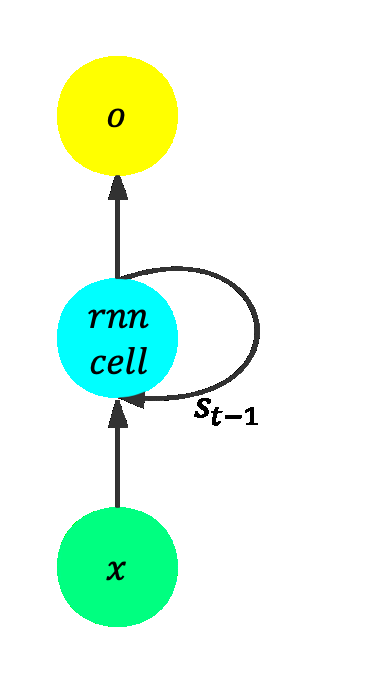
\includegraphics[width=0.15\textwidth]{./figs/rnncell.eps}\label{fig:rnncell}
%\caption{fig1}
}
\quad
\quad \quad \quad \quad
\subfigure[]{
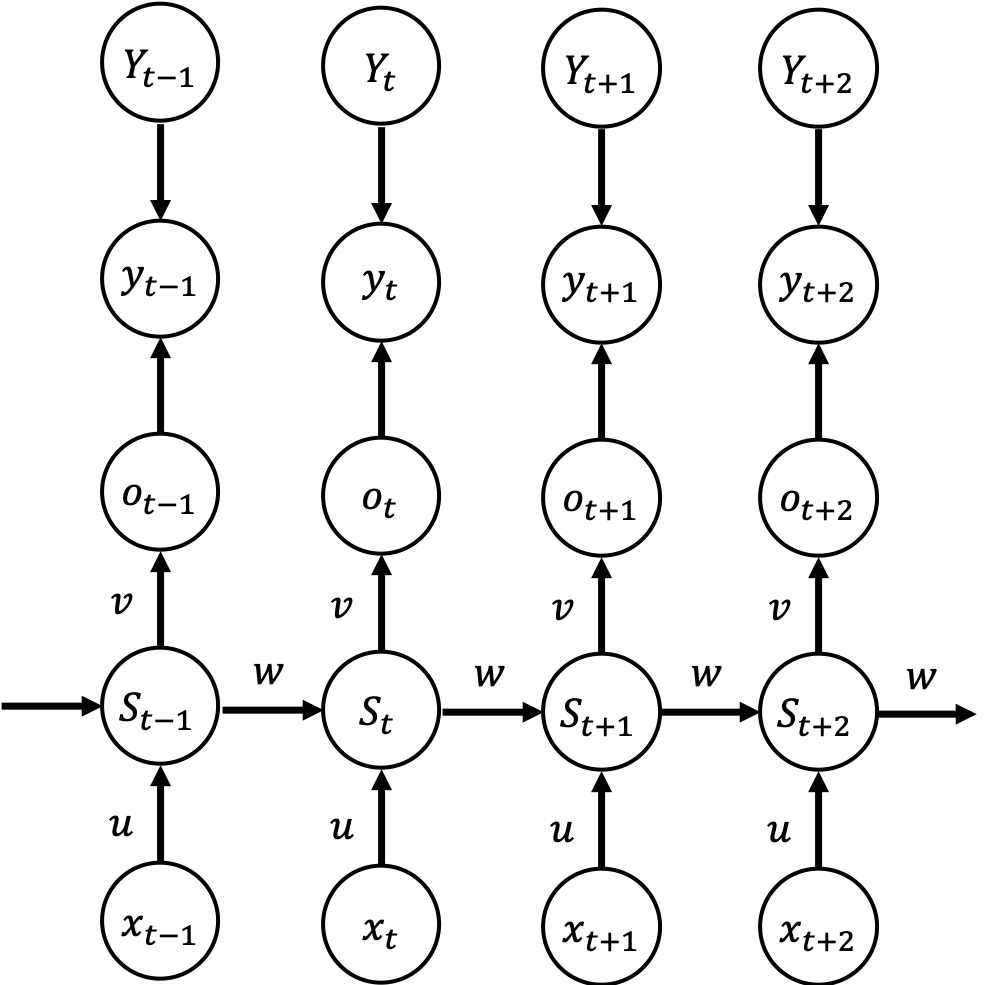
\includegraphics[width=0.27\textwidth]{./figs/unfold.png}\label{fig:unfold}
}
\caption{Two different forms of RNN. \textbf{a}: The typical RNN cell. \textbf{b}: The unfolded form of Fig.~\ref{fig:rnncell}, which is functionally identical to the original form~\cite{goodfellow2016deep}.}
\end{figure*}

\section{Related Work}\label{sec:related_work}
The fundamental research about Recurrent Neural Networks was published in the 1980s.
RNNs are powerful to model problems with a defined order but no clear concept of time, with a variant of Long short-term memory(LSTM)~\cite{hochreiter1997long}. 
In~\cite{bengio1994learning}, they argued that it was difficult to train RNN models due to the \textit{vanishing gradients} and \textit{exploding gradients}.
Moreover, since RNN is sensitive to the initialization of weights and bias, those parameters should be initialized according to the input data~\cite{sutskever2013importance}. In \cite{pascanu2013difficulty}, they also state some difficulties in train RNNs. There is still a lack of a method to solve these above problems in RNN at the same time until now.

ADMM was first introduced in~\cite{gabay1976dual}.
Its convergence was established in~\cite{gabay1983augmented,glowinski1989augmented}.
Since ADMM can decompose large problems with constraints into several small ones, it has been one of the most powerful optimization frameworks. It shows a multitude of well-performed properties in plenty of fields, such as machine learning~\cite{boyd2011distributed}, signal processing~\cite{sun2018iteratively} and tensor decomposition~\cite{goldfarb2014robust} and modal decomposition~\cite{masuyama2018modal}.

In general, ADMM seeks to tackle the following problem:
\begin{equation}\label{general ADMM}
\min\limits_{x,y} f(x) + g(y),     \quad {\rm s.t.} \quad Ax+By = c.
\end{equation}
Here, $f: \mathbb{R}^{n_1} \rightarrow \mathbb{R} $ and $g: \mathbb{R}^{n_2} \rightarrow \mathbb{R}$ are usually assumed to be convex functions.
In Eq.~\eqref{general ADMM}, $A \in \mathbb{R}^{m \times n_1}$, $B \in \mathbb{R}^{m \times n_2}$, $c \in \mathbb{R}^m$, and $Ax+By = c$ is a linear constraint and $n_1$, $n_2$ are the dimensions of $x$, $y$ respectively.
It is solved by the Augmented Lagrangian Method which is formalized as: 
\begin{equation}\label{equ:into}
\begin{aligned}
    \mathcal{L}_\beta(x, y, \lambda) = & f(x) + g(y) + <\lambda, Ax+By-c>     \\
                                     & + \frac{\beta}{2}\|Ax+By-c\|^2,
\end{aligned}
\end{equation}
where $\beta$ is the penalty term, $\lambda$ is the Lagrangian multiplier.

\tabcolsep 12pt
%\cmidrule(l){2-4}%
\renewcommand\arraystretch{1.3}
\begin{center}
{\footnotesize{\bf Table 1.} \textcolor{red}{I}mportant \textcolor{red}{N}otations and \textcolor{red}{C}orresponding \textcolor{red}{D}escriptions.}\\
\vspace{2mm}
\footnotesize{
\begin{tabular*}{\linewidth}{c c}\hline\hline\hline
Notations    & Descriptions  \\
\hline
$t$         & the timestep         \\
$x_t$       & the input of RNN cells    \\
$o_t$       & the output of RNN cells    \\
$s_t$        & the state at timestep $t$    \\
$u$            & the weight corresponding to the input     \\
$w$            & the weight corresponding to the state     \\
$y_t$        & the prediction at timestep $t$   \\
$N$            & the cell numbers after unfolding   \\
$R$            & the loss function     \\
$\Omega(w)$    & the regularization term    \\
$\theta$    & $\{u,w,b,a,s,v,c,o\}$ \\
$k$         & the iteration count       \\
\hline\hline\hline
\end{tabular*}%\vspace*{.2mm}
%\\\vspace{1mm}\parbox{8.3cm}{Note: You may explain the meaning of some special format, e.g., in bold, and/or give the full names of the abbreviations used in the table whose full names have not presented in the text.}
}
\label{tab:hyper acc}
\end{center}

Since ADMM was first proposed, plenty of theoretical and practical works have been developed in recent years~\cite{monteiro2010iteration}.
In 2016,~\cite{taylor2016training} proposed a new method to train neural networks using ADMM. They abandoned traditional optimizers and adopted ADMM, which trains neural networks in a robust and parallel fashion. 
Furthermore,  ADMM was applied to deep learning and obtained a remarkable result~\cite{wang2019admm}. They provided a gradient-free method to train neural networks, which gains convergent and great performance. Both of their works prove that ADMM is a powerful optimization method for neural networks because of its gradient-free property. However, RNNs are not as simple as a Multilayer Perceptron. The recurrent state brings many challenges when solving RNN with ADMM. 

\section{ADMM for RNNs}\label{sec:ADMM_RNN}
\subsection{Notation}\label{subsec:notions}
Before we dive into the ADMM methods for RNNs, we establish notations in this work.
Considering a simple RNN cell as shown in Fig.~\ref{fig:rnncell}, at timestep $t>=1$, $x_t$ is the input of the RNN cell and $o_t$ is the related output, RNNs could be expressed as:
\begin{equation}
\begin{array}{cl}
&\Phi(x_1, x_2, \cdots, x_N, u, v, w, b, c) \\
=& vf(ux_N+ w(vf(ux_{N-1}+ w(\cdots vf(ux_0 \\
& +b) + c \cdots)+b) + c)+b) + c\\
&+\Omega(W),
\end{array}
\end{equation} 
where $f(\cdot)$ is an activation function and $v, u, w, b$ and ${c}$ are learnable parameters, $s_0=0$. These parameters are also unified. The recurrent state in RNNs varies over timesteps as well as iterations, which brings difficulties to applying ADMM into RNNs directly. We adopt an unfolding form of RNN unit shown in Fig.~\ref{fig:unfold} and decouple these above parameters into three sub-problems.
Normally, at timestep $t$, the updates are listed in the following:
\begin{equation}
\begin{aligned}
    a_t & = ux_t + ws_{t-1} + b ,     \\
    s_t & = f(a_t)  ,                \\
    o_t & = vs_t + c ,               \\
%    y_t & = \textnormal{softmax}(o_t),   
\end{aligned}
\end{equation}
where $f(\cdot)$ is the activation function, such as ReLU~\cite{nair2010rectified}
or \textit{tanh}, usually \textit{tanh} in RNNs.
Important notations are summarized in Table~1. 
% Technically, Fig.~\ref{fig:rnncell} is generally considered as which is shown in Fig.~\ref{fig:unfold}.
% It is an unfolding form of the RNN cell in Fig.~\ref{fig:rnncell}.
In this paper, we consider RNN in an unfolding form and present a theoretical analysis based on it. 

For the sake of convenience, we define $\theta=\{u,w,b,a,s,v,c,o\}$ in the sequel. 
In term of applying ADMM into RNNs, assuming the RNN cell is unfolded into $N$ continuous cells, we try to solve the mathematical problem as follows:
\begin{problem}\label{problem:1}
\begin{equation}\label{equ:problem1}
\begin{aligned}
    & \min\limits_{\theta_t} \Phi(\theta_t) \equiv R(\theta_t) + \Omega(w) ,   \\
    & {\rm{s.t.}} \quad a_t = ux_t + ws_{t-1} + b, s_t = f(a_t), o_t = vs_t + c.
\end{aligned}
\end{equation}
\end{problem}
In Problem~\ref{problem:1}, $R(\theta_t)$ is the loss function which is convex and continuous, $\Omega(w)$ is the regularization term on the parameter $w$.
It is also a convex and continuous function.
Rather than solving Problem~\ref{problem:1} directly, we can relax it by adding an $l_2$ penalty term and transform Eq.~\eqref{equ:problem1} into 
\begin{problem}\label{problem:2}
\begin{equation}\label{equ:problem2}
    \begin{aligned}
        \min\limits_{\theta_t} & R(\theta_t) + \Omega(w) + \frac{\nu}{2}\sum_{t=1}^{N-1}(\|a_t-ux_t-ws_{t-1}-b\|^2   \\
        & + \|s_t-f(a_t)\|^2 + \|o_t-vs_t-c\|^2)  \\
    \end{aligned}
\end{equation}
\begin{equation}\nonumber
    \begin{aligned}
        {\rm{s.t.}} \quad a_N = ux_N + ws_{N-1} + b, s_N = f(a_N), o_N = vs_N + c,
    \end{aligned}    
\end{equation}
\end{problem}
where $\nu$ is a tuning parameter.
Compared with Problem~\ref{problem:1}, Problem~\ref{problem:2} is much easier to solve.
According to~\cite{wang2019admm}, the solution of Problem~\ref{problem:2} tends to be the solution of Problem~\ref{problem:1} when $\nu \rightarrow \infty$.
For simplicity and clarity, we often use $<\cdot,\cdot>$ to denote the inner product and $\Tilde{k} = k+1$.
For a positive semidefinite matrix $G$, we define the $G-$norm of a vector as $\|x\|_G=\|G^{1/2}x\|_2=\sqrt{x^TGx}$.

\subsection{ADMM Solver for RNN}\label{subsec:admm solver}
As aforementioned in Section~\ref{sec:related_work}, we explain that ADMM utilizes the Augmented Lagrangian Method to solve problems like Eq.~\eqref{equ:into}.
Similarly, we adopt the same way and present the corresponding Lagrangian function of Eq.~\eqref{equ:problem2}, namely Eq.~\eqref{equ:lagrangian}:
\begin{equation}\label{equ:lagrangian}
    \mathcal{L}_{\rho_1,\rho_2,\rho_3}(\theta)=R(o) + \Omega(w)+\phi(\theta_t),
\end{equation}
where $\phi(\theta_t)$ is defined in Eq.~\eqref{equ:phi}.
\begin{equation}\label{equ:phi}
    \begin{aligned}
        \phi(\theta_t) =&\frac{\nu}{2}\sum_{t=1}^{N-1}(\|a_t-ux_t-ws_{t-1}-b\|^2 + \|s_t-f(a_t)\|^2  \\   
        &  +\|o_t-vs_t-c\|^2) + <\lambda_1, a_N - ux_N - ws_{N-1}   \\
        &   - b> + <\lambda_2, s_N - f(a_N)> + <\lambda_3, o_N- \\ 
        & vs_N - c> + \frac{\rho_1}{2}\| a_N - ux_N - ws_{N-1} - b\|^2 +   \\
        &  \frac{\rho_2}{2}\|s_N - f(a_N)\|^2 + \frac{\rho_3}{2}\|o_N - vs_N -c\|^2.
    \end{aligned}
\end{equation}
Problem~\ref{problem:2} is separated into eight subproblems and could be solved through the updates of these parameters in $\theta_t$. Note that $u,w,b,v,c$ in $\theta$ are not changed over timestep $t$. Consequently, these parameters are supposed to update over iterations. To make it clear, we only describe the typical update rules for $u, a$ and $s$ in the following subsections because there are some useful and typical skills in these subproblems while analysis of the other parameters detailed in Appendix~\ref{appendix A} is similar.

\subsubsection{Update $u$}\label{sec:update_u}
We begin with the update of $u$ in Eq.~\eqref{equ:lagrangian} at iteration $k$.
In Eq.~\eqref{equ:phi}, $u$ and $x_t$ are coupled.
As a result, we need to calculate the pseudo-inverse of the (rectangular) matrix $x_t$, making it harder for the training process.
In order to solve this problem, we define $\textbf{G}=rI_{d}-\rho_1 x_{t}^Tx_{t}$ and replace it with Eq.~\eqref{equ:g-norm_u}. 
\begin{equation}\label{equ:g-norm_u}
\begin{aligned}
    u^{\Tilde{k}} \leftarrow & \arg\min \frac{\nu}{2}\sum_{t=1}^{N-1}\|a_t-ux_t-ws_{t-1}-b\|^2+\frac{\rho_1}{2}\|a_N \\
    & -ux_N-ws_{N-1}-b-\lambda_1/\rho_1\|^2+\frac{N}{2}\|u-u^k\|_{\textbf{G}}^2.   \\
\end{aligned}
\end{equation}
It is equivalent to the linearized proximal point method inspired by~\cite{rockafellar1976monotone}:
\begin{equation}\label{equ:update_ut}
    \begin{aligned}
        u^{\Tilde{k}} \leftarrow & \arg\min \frac{Nr}{2}\|u-u^k\|^2+\nu(u-u^k)^T\sum_{t=1}^{N-1}[(x_t^k)^T   \\
        & (a_t-u^kx_t^k-w^ks_{t-1}^k-b^k)]+\rho_1(u-u^k)^T[(x_N^k)^T   \\
        & (a_N^k-u^kx_N^k-w^ks_{N-1}^k-b^k-\lambda_1^k/\rho_1)].  \\
    \end{aligned}
\end{equation}
In this way, the update of $u$ is greatly sped up than the vanilla ADMM. It is worth noting that $r$ needs to be set properly and $r$ could also affect the performance of ADMMiRNN. 

\subsubsection{Update $a$}

Adding a proximal term similar to that in Section~\ref{sec:update_u}, if $t<N$, this could be done by
\begin{equation}\label{equ:update_at}
    \begin{aligned}
        a_t^{\Tilde{k}} \leftarrow & \arg\min \frac{r}{2}\|a_t-a_t^k\|^2+\nu (a_t-a_t^k)^T(a_t^k-u^kx_t^k \\
        & -w^ks_{t-1}^k-b^k)+\frac{\nu}{2}\|s_t-f(a_t)\|^2.
    \end{aligned}
\end{equation}
When $t=N$, 
\begin{equation}\label{equ:update_aN}
    \begin{aligned}
        a_N^{\Tilde{k}} \leftarrow & \arg\min \frac{r}{2}\|a_N-a_N^k\|^2+\rho_{1} (a_N-a_N^k)^T(a_N^k-u^kx_N^k  \\
        & -w^ks_{N-1}^k-b^k-\lambda_1/\rho_1)+\frac{\rho_{2}}{2}\|s_N-f(a_N)-\lambda_2/\rho_2\|^2. \\
    \end{aligned}
\end{equation}
% Here is a \textbf{trick}:
% If $a_t$ is small enough, we have $f(a_t)=a_t$ as a result of the property of \textit{tanh} function. In this way, we could simplify the calculation of $a_t$.

\subsubsection{Update $s$}
The parameter $s$ represents the hidden state in the RNN cell shown in Fig.\ref{fig:rnncell}.
With regard to the update of $s$, there are $s_{t-1}$ and $s_t$ in Eq.~\eqref{equ:phi}.
However, we only consider $s_t$ in the RNN model. 
It is because $s_{t-1}$ has been updated in last unit and would cause calculation redundancy in the updating process. This is another \textbf{trick} in our solution. 
Besides, $s_t$ also needs to be decoupled with $w$. 

If $t<N$, we could update $s_t$ through
\begin{equation}\label{equ:update_st}
    \begin{aligned}
        s_t^{\Tilde{k}} \leftarrow & \arg\min \frac{r}{2}\|s_t-s_t^k\|^2+\nu(s_t-s_t^k)^T[(v^k)^T(o_t^k-v^ks_t^k\\
        & -c^k)]+\frac{\nu}{2}\|s_t-f(a_t)\|^2.   \\
    \end{aligned}    
\end{equation}
And when $t=N$, 
\begin{equation}\label{equ:update_sN}
    \begin{aligned}
        s_N^{\Tilde{k}} \leftarrow & \arg\min \frac{r}{2}\|s_N-s_N^k\|^2+\rho_3(s_N-s_N^k)^T[(v^k)^T(o_N^k-\\
        & v^ks_N^k-c^k-\lambda_3^k/\rho_3)].   \\
    \end{aligned}    
\end{equation}


\subsubsection{Update Lagrangian Multipliers}
Similar to the parameters update, $\lambda_1$, $\lambda_2$ and $\lambda_3$ are updated as follows respectively:
\begin{subequations}
\begin{equation}\label{equ:update_lambda1}
    \lambda_1^{\Tilde{k}} = \lambda_1^k + \rho_1(a_N-ux_N-ws_{N-1}-b),
\end{equation}
\begin{equation}\label{equ:update_lambda2}
    \lambda_2^{\Tilde{k}} = \lambda_2^k + \rho_2(s_N-f(a_N)),
\end{equation}
\begin{equation}\label{equ:update_lambda3}
    \lambda_3^{\Tilde{k}} = \lambda_3^k + \rho_3(o_N-vs_N-c).
\end{equation}
\end{subequations}




\begin{algorithm}[H]
\caption{The training algorithm for ADMMiRNN.}
\label{alg:RNN algorithm}
\textbf{Input}: iteration $K$, input $x$, timestep $N$. \\
\textbf{Parameter}: $u$, $w$, $b$, $v$, $c$, $s_0$, $\lambda_1$, $\lambda_2$, and $\lambda_3$\\
\textbf{Output}: $u$, $w$, $b$, $v$, $c$,
\begin{algorithmic}[1] %[1] enables line numbers
\STATE Initialize $k=0$, $u$, $w$, $b$, $v$, $c$, $s_0$, $\lambda_1$, $\lambda_2$, and $\lambda_3$.
\FOR{$k=1,2,\cdots, K$}
\FOR{$t=1,2,\cdots, N$}
\IF{$t<N$} 
    \STATE Update $o_t^{\Tilde{k}}$ in Eq.~\eqref{equ:update_ot}.
\ELSIF{$t=N$}
    \STATE Update $o_N^{\Tilde{k}}$ in Eq.~\eqref{equ:update_oN}.
\ENDIF
    \STATE Update $c^{\Tilde{k}}$ in Eq.~\eqref{equ:update_ct}.
    \STATE Update $v^{\Tilde{k}}$ in Eq.~\eqref{equ:update_vt}.
\IF{$t<N$} 
    \STATE Update $s_t^{\Tilde{k}}$ in Eq.~\eqref{equ:update_st}.
    \STATE Update $a_t^{\Tilde{k}}$ in Eq.~\eqref{equ:update_at}.
\ELSIF{$t=N$}
    \STATE Update $s_N^{\Tilde{k}}$ in Eq.~\eqref{equ:update_sN}.
    \STATE Update $a_N^{\Tilde{k}}$ in Eq.~\eqref{equ:update_aN}.
\ENDIF
    \STATE Update $b^{\Tilde{k}}$ in Eq.~\eqref{equ:update_bt}.
    \STATE Update $w^{\Tilde{k}}$ in Eq.~\eqref{equ:update_w}.
    \STATE Update $u^{\Tilde{k}}$ in Eq.~\eqref{equ:update_ut}.
    \STATE Update $u^{\Tilde{k}}$ in Eq.~\eqref{equ:update_ut}.
    \STATE Update $w^{\Tilde{k}}$ in Eq.~\eqref{equ:update_w}.
    \STATE Update $b^{\Tilde{k}}$ in Eq.~\eqref{equ:update_bt}.
\IF{$t<N$} 
    \STATE Update $a_t^{\Tilde{k}}$ in Eq.~\eqref{equ:update_at}.
    \STATE Update $s_t^{\Tilde{k}}$ in Eq.~\eqref{equ:update_st}.
\ELSIF{$t=N$}
    \STATE Update $a_N^{\Tilde{k}}$ in Eq.~\eqref{equ:update_aN}.
    \STATE Update $s_N^{\Tilde{k}}$ in Eq.~\eqref{equ:update_sN}.
\ENDIF    
    \STATE Update $v^{\Tilde{k}}$ in Eq.~\eqref{equ:update_vt}.
    \STATE Update $c^{\Tilde{k}}$ in Eq.~\eqref{equ:update_ct}.
\IF{$t<N$}    
    \STATE Update $o_t^{\Tilde{k}}$ in Eq.~\eqref{equ:update_ot}.
\ELSIF{$t=N$}
    \STATE Update $o_N^{\Tilde{k}}$ in Eq.~\eqref{equ:update_oN}.
\ENDIF
\ENDFOR
\STATE Update $\lambda_1^{\Tilde{k}}$ in Eq.~\eqref{equ:update_lambda1}.
\STATE Update $\lambda_2^{\Tilde{k}}$ in Eq.~\eqref{equ:update_lambda2}.
\STATE Update $\lambda_3^{\Tilde{k}}$ in Eq.~\eqref{equ:update_lambda3}.
\ENDFOR
\STATE \RETURN $u$, $w$, $b$, $v$, $c$,
\end{algorithmic}
\end{algorithm}




\subsubsection{Algorithm}
Generally, we update the above parameters in two steps.
First, these parameters are update in a backward way, namely $o\rightarrow c \rightarrow v \rightarrow s \rightarrow a \rightarrow b \rightarrow w \rightarrow u$.
Afterwards, ADMMiRNN reverses the update direction in $u\rightarrow w \rightarrow b \rightarrow a \rightarrow s \rightarrow v \rightarrow c \rightarrow o$.
After all those variables in an RNN cell update, the Lagrangian multipliers then update. Proceeding with the above steps, we could arrive at the algorithms for ADMMiRNN, which is outlined in Algorithm~\ref{alg:RNN algorithm}.


\subsection{Paralleled Algorithms}\label{sec:paralleled algorithms}


\begin{figure*}[tbp]
\centering
\subfigure[SP-ADMMiRNN.]{
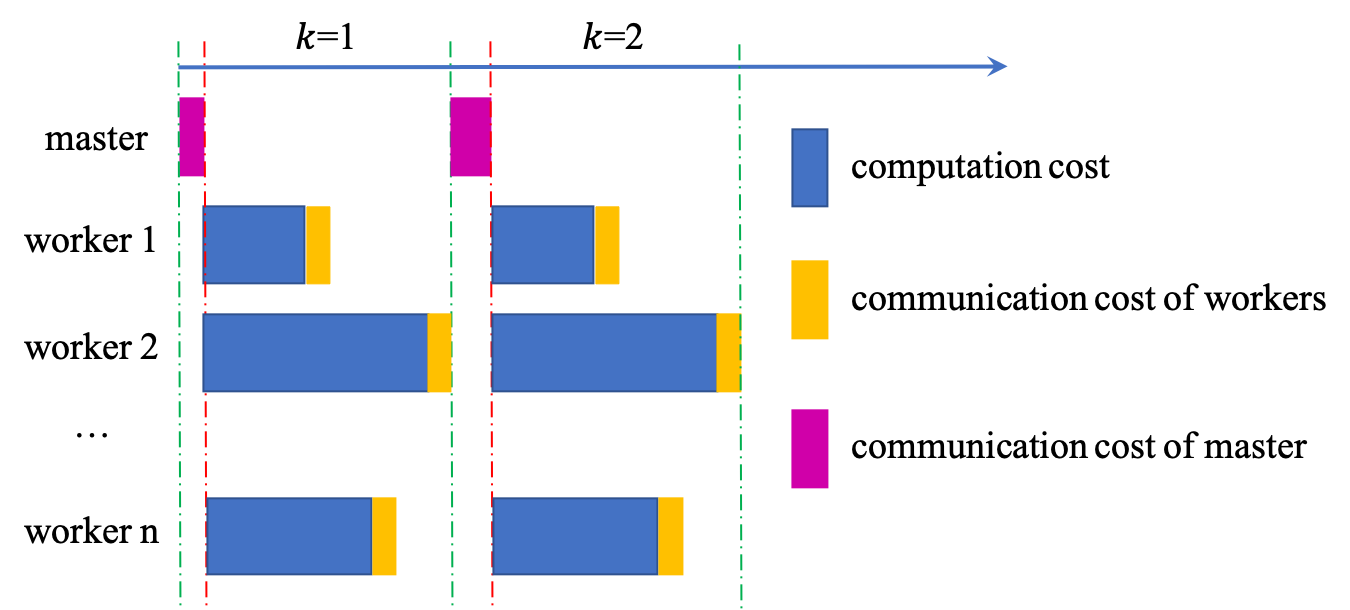
\includegraphics[width=0.45\textwidth]{./figs/sp.eps}\label{fig:sync parallel}
}
\subfigure[AP-ADMMiRNN.]{
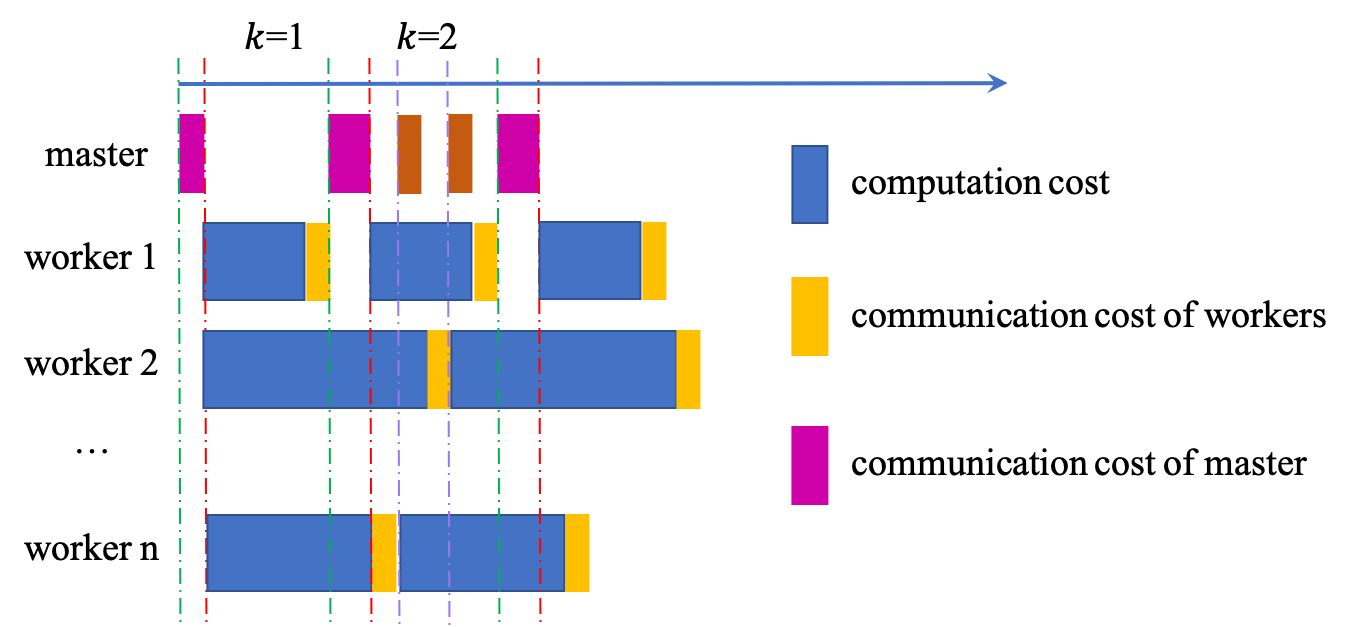
\includegraphics[width=0.45\textwidth]{./figs/ap.eps}\label{fig:async parallel}
}
\caption{Illustration of Synchronous and Asynchronous Paralleled ADMMiRNN.}\label{fig:sync and async}
\end{figure*}

In this section, we introduce the distributed training algorithms in ADMMiRNN, including Asynchronous Parallel ADMMiRNN~(AP-ADMMiRNN) and Synchronous Parallel ADMMiRNN~(SP-ADMMiRNN). 
In our distributed algorithms, we adopt a ``\textit{master-worker}'' method. The \textit{master} is responsible for the initialization of parameters and managing those parameters while the \textit{worker} does all the calculations in ADMMiRNN. So the algorithm of the \textit{master} in AP-ADMMiRNN and SP-ADMMiRNN could both be presented in Algorithm~\ref{alg:master}.  
\begin{algorithm}[H]
\caption{The master in AP-ADMMiRNN and SP-ADMMiRNN.} \label{alg:master}
\hspace*{0.02in} 
\textbf{Input:} the iteration number $K$, input data $x$, send queue $Q_s$, receive queue $Q_r$. \\
\hspace*{0.02in}  
\textbf{Output:} $loss$ and $accuracy$.\\
\begin{algorithmic}[1]
\STATE Init: $u, w, s_0, b, v, c$.
\STATE $Q_s$ sends all the hyperparameters to workers.
	\STATE $Q_s$ sends $u, w, s_0 b, v, c$ to workers.
\FOR{t = 1 to $K$} 
	\STATE $Q_r$ receives $u, w, s_{t}, b, v, c$ from workers.
	\STATE Compute $loss$ and $accuracy$.
\ENDFOR
\RETURN $loss$ and $accuracy$.
\end{algorithmic}
\end{algorithm}

\begin{algorithm}[H]
\caption{The worker algorithms in SP-ADMMiRNN.} \label{alg:sp-admmirnn worker}
\hspace*{0.02in} 
\textbf{Input:} the worker number $N_{sp}$, send queue $Q_s$, receive queue $Q_r$. \\
\hspace*{0.02in}  
\textbf{Output:} $u, w, s_{t}, b, v, c$.  \\
\begin{algorithmic}[1]
\STATE $Q_r$ receives hyperparameters from the master.  
\STATE $Q_r$ receives $u, w, s_{t}, b, v, c$ from the master.
\STATE Assign all the parameters to $N_{sp}$ workers. 
\FOR{t = 1 to $K$} 
    \FOR{i = 1 to $N_{sp}$}
        \STATE worker $N_i$ updates its parameters.
    \ENDFOR
	\STATE $Q_s$ sends $u, w, s_{t}, b, v, c$ to master.
\ENDFOR
% \RETURN $loss$ and $accuracy$.
\end{algorithmic}
\end{algorithm}

\begin{algorithm}[H]
\caption{The worker algorithms in AP-ADMMiRNN.} \label{alg:ap-admmirnn worker}
\hspace*{0.02in} 
\textbf{Input:} the worker number $N_{ap}$, send queue $Q_s$, receive queue $Q_r$. \\
\hspace*{0.02in}  
\textbf{Output:} $u, w, s_{t}, b, v, c$.\\
\begin{algorithmic}[1]
\STATE $Q_r$ receives hyperparameters from the master.  
\STATE $Q_r$ receives $u, w, s_{t}, b, v, c$ from the master.
\STATE Assign all the parameters to $N_{ap}$ workers. 
\FOR{t = 1 to $K$} 
    \FOR{i = 1 to $N_{ap}$}
        \STATE worker $N_i$ updates its parameters.
        \STATE $Q_s$ sends those updated parameters to the master.
    \ENDFOR
	\STATE $Q_s$ sends $u, w, s_{t}, b, v, c$ to master.
\ENDFOR
% \RETURN $loss$ and $accuracy$.
\end{algorithmic}
\end{algorithm}

In SP-ADMMiRNN, all the workers calculate parts of updates of those parameters. The worker algorithms are summarized in Algorithm~\ref{alg:sp-admmirnn worker}. At first, the worker receives all the hyperparameters and parameters form the master. And then these parameters would be assigned to $N_{sp}$ workers. After all those parameters are updated, they would be sent to master through the send queue $Q_s$ in worker.
 
As for AP-ADMMiRNN, its worker algorithms are presented in Algorithm~\ref{alg:ap-admmirnn worker}. Algorithm~\ref{alg:ap-admmirnn worker} is slightly different from Algorithm~\ref{alg:sp-admmirnn worker} in Line 7. The send queue $Q_s$ in AP-ADMMiRNN would send those parameters whichever has been updated. In this way, the convergence could speed up a lot. 

Fig.\ref{fig:sync and async} shows the detailed process of SP-ADMMiRNN and AP-ADMMiRNN. In SP-ADMMiRNN, the training time depends on the longest computation time. The other workers need to wait for the most time consuming worker. It is clear that in SP-ADMMiRNN the master takes a lot of time waiting for the parameters in each iterations. However, in AP-ADMMiRNN, the parameters could be sent to the master as long as they are updated, which saves a lot of unnecessary time. The master is much busier than that in SP-ADMMiRNN.


\subsection{Convergence Analysis}
In this section, we present the convergence analysis about ADMMiRNN. For convenience, we define $\rho=\{\rho_1, \rho_2, \rho_3\}$. First, we give some mild assumptions as follows:
% \begin{assumption}
\begin{figure*}[tb]
\centering
\subfigure[training loss versus iterations.]{
\includegraphics[width=0.46\textwidth]% , height=14em]
{./figs/train_loss.eps}\label{fig:train_loss comparison}
}
\subfigure[test loss versus iterations.]{
\includegraphics[width=0.46\textwidth]% , height=14em]
{./figs/test_loss.eps}\label{fig:test_loss comparison}
}
\caption{Training loss and test loss versus iterations of RNN via ADMM, SGD, AdaGrad, Momentum, RMSprop, and Adam. ADMMiRNN achieves the best performance against other optimizers on MNIST.}\label{fig:comparison}
%    \vspace{-1em}
\end{figure*}

{\bf Assumption 1.}\label{assumption:1} The gradient of $R$ is $H$-\textit{Lipschitz} continuous, $i.e.$, $\| \nabla R(o_1) - \nabla R(o_2)\| \le H\|o_1 - o_2\|$, $H \ge 0$ and is called the \textit{Lipschitz constant}. 
This is equivalent to $R(o_1) \le R(o_2) + \nabla R(o_2)\cdot (o_1 - o_2) + H/2\|o_1-o_2\|^2$;
% \end{assumption}
% \begin{assumption}

{\bf Assumption 2.} The gradient of the objective function $\mathcal{L}_\rho$ is bounded, $i.e.$, there exists a constant $C$ such that $\nabla \mathcal{L}_\rho \le C$;
% \end{assumption}
% \begin{assumption}

{\bf Assumption 3.} The second-order moment of the gradient $g_t$ is uniformly upper-bounded, that is to say $\mathbb{E}\|g_t\|^2 \le C$.
% \end{assumption}

Such assumptions are typically used in~\cite{Saeed1,Saeed2,zou2019sufficient}.
Under these assumptions, we will have the properties~\cite{wang2019multi} shown in the supplementary materials. Then we can prove that ADMMiRNN converges under the following theorems.
% \begin{theorem}

{\bf Theorem 1.} If $\rho_i > 2H~(i=1,2,3)$ and \textbf{Assumption1-3} hold, then \textbf{Property 1-3} in the supplementary materials hold. 

{\bf Theorem 2.} If $\rho_i > 2H~(i=1,2,3)$, for the variables $(\theta, \lambda_1, \lambda_2, \lambda_3)$ in Problem~\ref{problem:2}, starting from any $(\theta^0, \lambda_1^0, \lambda_2^0, \lambda_3^0)$, it at least has a limit point $(\theta^*, \lambda_1^*, \lambda_2^*, \lambda_3^*)$ and any limit point $(\theta^*, \lambda_1^*, \lambda_2^*, \lambda_3^*)$ is a critical point of Problem~\ref{problem:2}. In other words, $0 \in \partial \mathcal{L}_{\rho_1,\rho_2,\rho_3}(\theta^*)$.
% \end{theorem}

Theorem~2 concludes that ADMMiRNN has a global convergence. 
% Its proof is also provided in the supplementary materials.

{\bf Theorem 3.} For a sequence $\theta$ generated by Algorithm~\ref{alg:RNN algorithm}, define $m_k=\min\limits_{0\le t \le k}(\|\theta^{\Tilde{k}}-\theta^k\|_2^2)$, the convergence rate of $m_k$ is $O(1/k)$.

Theorem~3 concludes that ADMMiRNN converges globally at a rate of $O(1/T)$. The convergence rate is consistent with the current work of ADMM~\cite{wang2019multi,zhong2014fast,ouyang2013stochastic}. 
Due to space limited, the proofs of the above theorems are also omitted in the supplementary materials.
These analysis is suitable for ADMMiRNN and SP-ADMMiRNN. 

When it comes to AP-ADMMiRNN, the convergence analysis is more complicated. 
This analysis is still based on former assumptions. From \cite{chang2016asynchronous}, we have the following lemma, 

{\bf Lemma 1.} There exists a constant $S \in [1, N]$ such that 
\begin{equation}
    \begin{aligned}
        \infty > & \mathcal{L}_{\rho}(\theta^{0}) - \Phi^{*} \ge 0,\\
        \rho_i > & \frac{(1+H+H^2)+\sqrt{(1+H+H^2)^2+8H^2}}{2} i=1,2,3,\\
    \end{aligned}
\end{equation}
where $\Phi^{*} > -\infty$ and is the optimal objective value of Problem~\ref{problem:1}. Then $\theta^t$ generated by Algorithm~\ref{alg:master} and Algorithm~\ref{alg:ap-admmirnn worker} are bounded and have limit points which satisfy KKT conditions of Problem~\ref{problem:2}.

Besides, in AP-ADMMiRNN, we need another additional assumption 4.

{\bf Assumption 4.} $R(o)$ is strongly convex with $\delta^2 > 0$.
\begin{figure*}[htbp]
\centering
\subfigure[training loss of ADMMiRNN and some typical optimizers.]{
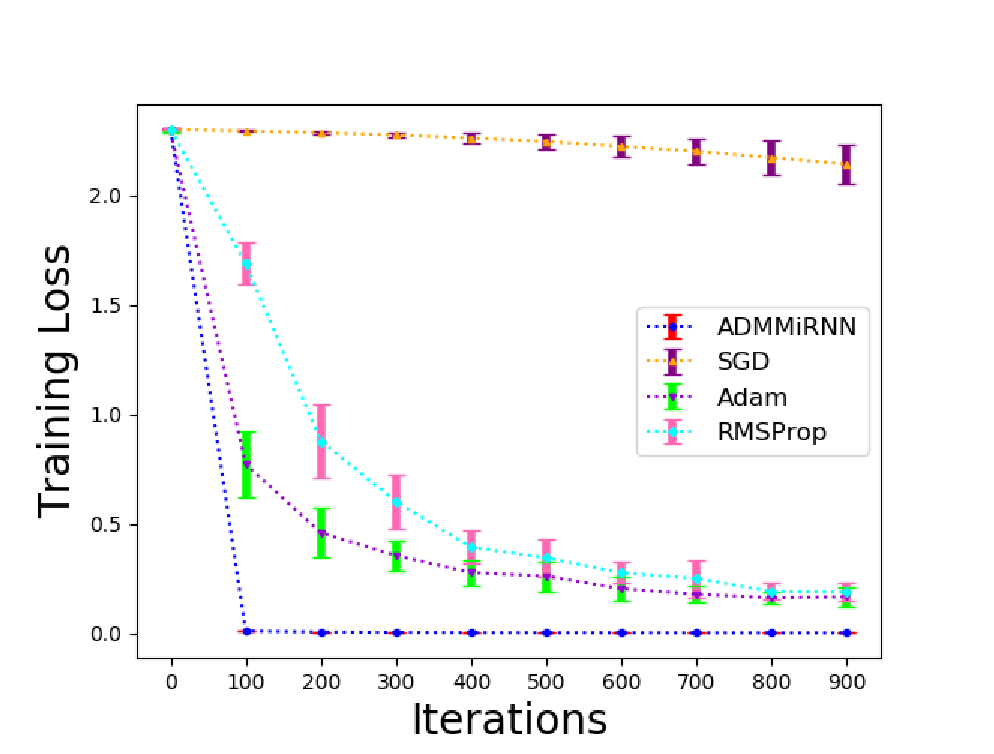
\includegraphics[width=0.46\textwidth, height=15em]{./figs/errorbar.eps}\label{fig:errbar_train}
}
\subfigure[test loss of ADMMiRNN and some typical optimizers.]{
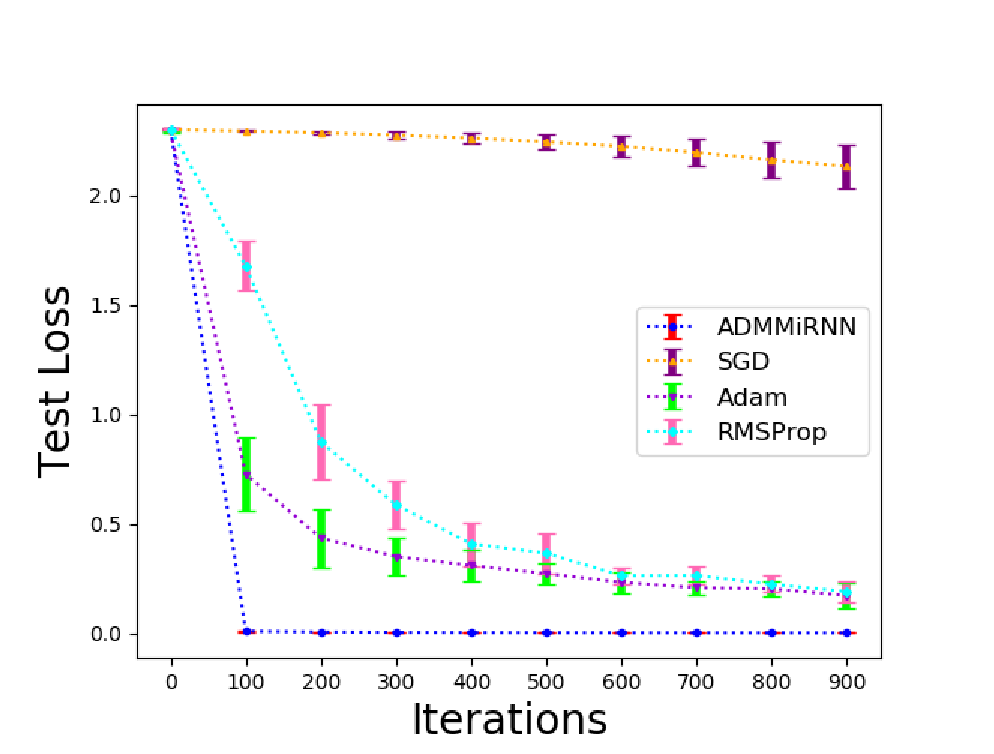
\includegraphics[width=0.46\textwidth, height=15em]{./figs/errorbar_test.eps}\label{fig:errbar_test}
}
\caption{The comparison of stability among ADMMiRNN, SGD, Adam and RMSProp. For each optimization method, we repeated experiments 10 times to obtain the mean and variance of the training loss and test loss against iterations on MNIST.}\label{fig:errorbar}
\end{figure*}

{\bf Theorem 4.} Let $\delta = 0$ and $0 < \rho_i \le \frac{\delta^2}{(5\tau -3)\max{2\tau, 3(\tau -1)}} (i=1,2,3)$ and $\theta^k$ is generated by Algorithm~\ref{alg:master} and Algorithm~\ref{alg:ap-admmirnn worker}. Then it holds that 
\begin{equation}
    \begin{aligned}
        \|\Phi(\theta^k) - \Phi(\theta)^{*} + \|\theta^k-\theta_0\| \le \frac{2+\sigma_{\lambda}C}{k}
    \end{aligned}
\end{equation}
Lemma 1 and Theorem 4 imply that Algorithm~\ref{alg:ap-admmirnn worker} is guaranteed to converge to the set of KKT points as long as $\rho_i (i=1,2,3)$ satisfy those conditions.
More details and proofs could be referred in \cite{chang2016asynchronous}.   

\section{Experiments}\label{sec:experiments}
\subsection{Setup}
We train a RNN model shown in Fig.\ref{fig:rnncell} on MNIST~\cite{lecun1998gradient} and IMDb~\cite{dodds2006popular}. 
This is achieved by NumPy and those parameters are updated in a manner of Algorithm~\ref{alg:RNN algorithm}.
The MNIST dataset has 55,000 training samples and 10,000 test samples and was first introduced in~\cite{lecun1998gradient} to train handwritten-digit image recognition. The IMDb dataset consists of 50,000 movie reviews~(half negative and the half positive). This dataset is spit evenly into 25,000 reviews for training and 25,000 reviews for testing. 
All the experiments related to MNIST are conducted in 1000 iterations on a 64-bit Ubuntu 16.04 system.

Furthermore, our experiments are also conducted on a text.
The text could also be accessed from our open-source code repository.
Training on a text is a typical RNN task.
We achieved a typical RNN model and unfolded it to $N$ cells with NumPy and $N$ is also the length of the input sequence. 
In our experiments, we adopt a kind of smooth loss.
These experiments are performed on a Macbook Pro with an Intel 3.1~GHz Core i5 Processor and 8~GB Memory. 

In our paralleled experiments, we train ADMMiRNN, SP-ADMMiRNN and AP-ADMMiRNN on MNIST in 30 iterations. Those experiments are performed on a Ubuntu-16 system, with 2 1080-Ti GPUs. 

In all of our experiments, we utilize a fixed value strategy for these hyperparameters, such as $\rho_1, \rho_2$ and $\rho_3$. 

\subsection{Convergence Results}
\subsubsection{Results on MNIST}
We train the simple RNN model shown in Fig.\ref{fig:rnncell} through different optimizers, including SGD, Adam, Momentum~\cite{qian1999momentum}, RMSProp~\cite{tieleman2012lecture} and AdaGrad~\cite{duchi2011adaptive}.
We compare our ADMMiRNN with these commonly-used optimizers in training loss and test loss and display our experimental results on MNIST in Fig.\ref{fig:train_loss comparison} and Fig.~\ref{fig:test_loss comparison} respectively.
Fig.~\ref{fig:train_loss comparison} and Fig.\ref{fig:test_loss comparison} indicate that ADMMiRNN converges faster than the other optimziers.
ADMMiRNN gets a more smooth loss curve while the loss curves of other optimizers shake a lot.
This means ADMMiRNN trains models in a relatively stable process.
Besides, ADMMiRNN gets a much more promising training loss and test loss.
These results not only prove that ADMMiRNN could converge in RNN tasks but also confirm that ADMMiRNN is a much powerful tool than traditional gradient-based optimizers in deep learning. 

\begin{center}
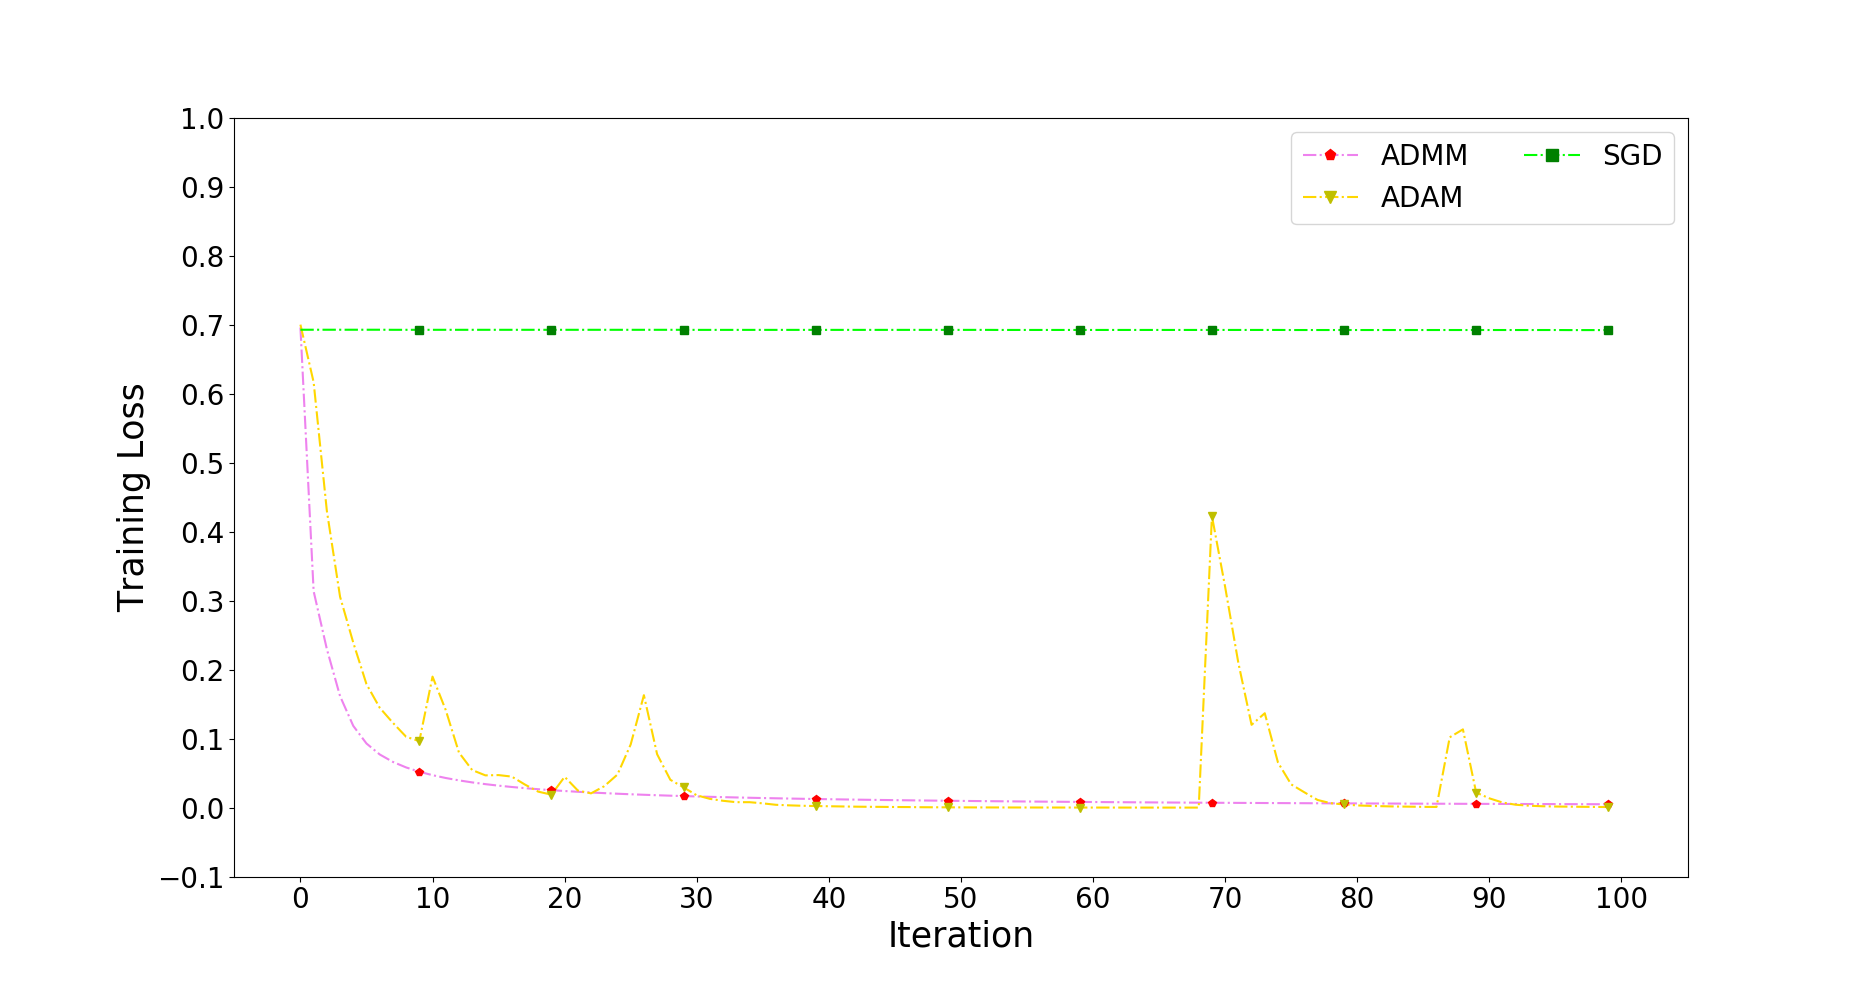
\includegraphics[width=0.46\textwidth, height=14em]{./figs/imdb_loss.eps}\\
\vspace{2mm}
\parbox[c]{8.3cm}{\footnotesize{Fig.5.~}  The training loss comparison of ADMMiRNN, SGD and Adam on IMDb.}%\vspace*{.2mm}
 \label{fig:length}
\end{center}
\subsubsection{Results on IMDb}
Fig.5 shows that our additional experiments comparing the training loss on IMDb of ADMMiRNN, SGD and Adam. From Fig.5, we find that ADDMiRNN converges faster than SGD and Adam as well as outperforms them, which is consistent with the trends in Fig.\ref{fig:comparison}. We notice that ADMMiRNN achieves a close result to Adam but there are several fluctuation in Adam while ADMMiRNN don't. However, SGD fails on this task. These results also illustrate that the performance and efficiency of ADMMiRNN. 

In our experiments on MNIST and IMDb, we find the accuracy of ADMMiRNN always reaches 1.0 within several iterations, which sometimes might be 2 or 3. According to our analysis, this is because in our method, we choose to solve the target directly instead of computing gradients, which speeds up the convergence and produces an intuitively better solution. 

\begin{center}
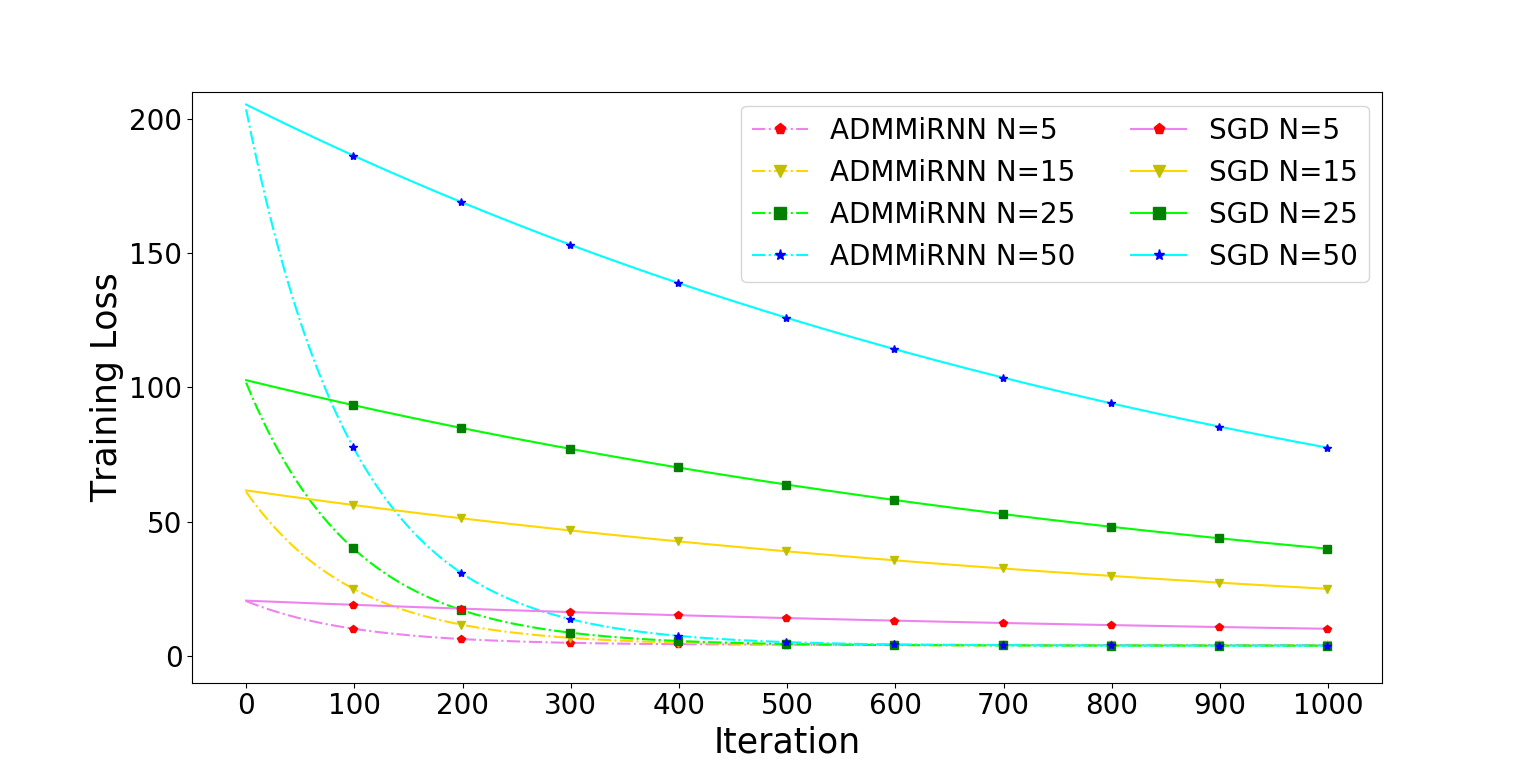
\includegraphics[width=0.46\textwidth, height=14em]{./figs/length.eps}\\
\vspace{2mm}
\parbox[c]{8.3cm}{\footnotesize{Fig.6.~}  The results of ADMMiRNN and SGD on different input sequence length. In this figure, $N$ represents the length.}%\vspace*{.2mm}
 \label{fig:length}
\end{center}
\subsubsection{Results on Text Data}
Besides experiments on MNIST, we also explore how ADMMiRNN performs in text classification tasks.
% In this section, we display our experiments on text data.
% We train a text with ADMMiRNN, SGD, RMSProp, respectively, in 400 iterations and display the results in Fig.~\ref{fig:rnn result}.
% From this picture, we can identify that ADMMiRNN converges faster than SGD and RMSProp.
% %However, it doesn't achieve the best result. This might be a result of some terrible hyperparameter values.
One critical shortcoming of current RNN models is that they are sensitive to the length of the input sequence because the longer the input sequence is, the worse training results are. To investigate the sensitivity of ADMMiRNN to the input length, we measure the performance of ADMMiRNN and SGD on the text data with different input sequence length. The results are displayed in Fig.6. Here, we adopt the average loss of the input sequence as our target. From Fig.6, we have evidence that ADMMiRNN always produces a remarkable result and is nearly immune to the length, which performs much more impressive than SGD regardless of the length of the input sequence.  

\tabcolsep 9pt
%\cmidrule(l){2-4}%
\renewcommand\arraystretch{1.3}
\begin{center}
{\footnotesize{\bf Table 2.} \textcolor{red}{T}raining \textcolor{red}{L}oss and \textcolor{red}{T}est \textcolor{red}{L}oss under \textcolor{red}{D}ifferent \textcolor{red}{H}yperparameter \textcolor{red}{S}ettings.}\\
\vspace{2mm}
\footnotesize{
\begin{tabular*}{\linewidth}{cccccc}\hline\hline\hline
$\rho_1$ & $\rho_2$ & $\rho_3$ & $r$ & training loss & test loss  \\
\hline
1 & 1 & 1 & 1       & $5.045\times10^{-2}$  & $5.046\times10^{-2}$   \\
0.1 & 1 & 1 & 1    & $5.339\times10^{-2}$  & $5.338\times10^{-2}$   \\
1 & 0.1 & 1 & 1     & $5.338\times10^{-2}$      & $5.340\times10^{-2}$     \\
1 &1 & 0.1 & 1   & $3.776\times10^{-4}$  & $3.776\times10^{-4}$      \\
1 &1 & 10  & 1            & $0.9984$  & $0.9985$     \\
% (1,1,100,1)  &  Nan   &  Nan    \\
1 & 1 & 1 & 10   &  $5.339\times10^{-2}$     &  $5.338\times10^{-2}$    \\
1 & 1 & 10 & 10         & $0.9987$   & $0.9986$      \\
\hline\hline\hline
\end{tabular*}%\vspace*{.2mm}
%\\\vspace{1mm}\parbox{8.3cm}{Note: You may explain the meaning of some special format, e.g., in bold, and/or give the full names of the abbreviations used in the table whose full names have not presented in the text.}
}
\label{tab:hyper loss}
\end{center}


\subsection{Stability}
As aforementioned, the initialization of weights and biases is critical in RNN models. 
In this section, we mainly compare ADMM with some different optimizers and explore its stability for RNN.
In brief, we compare ADMMiRNN with SGD, Adam, and RMSProp and repeat each scheme ten times independently.
% In order to present a clear comparison, every 100 iterations, we get one data and compute their average and standard deviation.
The experimental results are displayed in Fig.\ref{fig:errorbar}.
The blocks in Fig.~\ref{fig:errbar_train} and Fig.~\ref{fig:errbar_test} represent the standard deviation of the samples drawn from the training and testing process.
The smaller the blocks are, the more stable the method is. 
From Fig.\ref{fig:errbar_train} and Fig.\ref{fig:errbar_test}, we observe that at the beginning, SGD has a small fluctuation. But as the training progresses, the fluctuation gets more and sharper, which means that SGD is tending to be unstable. 
As for Adam and RMSProp, their variance is getting smaller, but still large with regard to ADMMiRNN. 
According to different initialization of weights and biases, these optimizers may cause different results within a big gap between them.
Specifically, ADMMiRNN has a relatively small variance from beginning to end compared with SGD, Adam and RMSProp, which is too small to show clearly in Fig.\ref{fig:errbar_train} and Fig.\ref{fig:errbar_test}, which indicates that ADMMiRNN is immune to the initialization of weights and biases and settle the sensitivity of RNN models to initialization.
\begin{center}
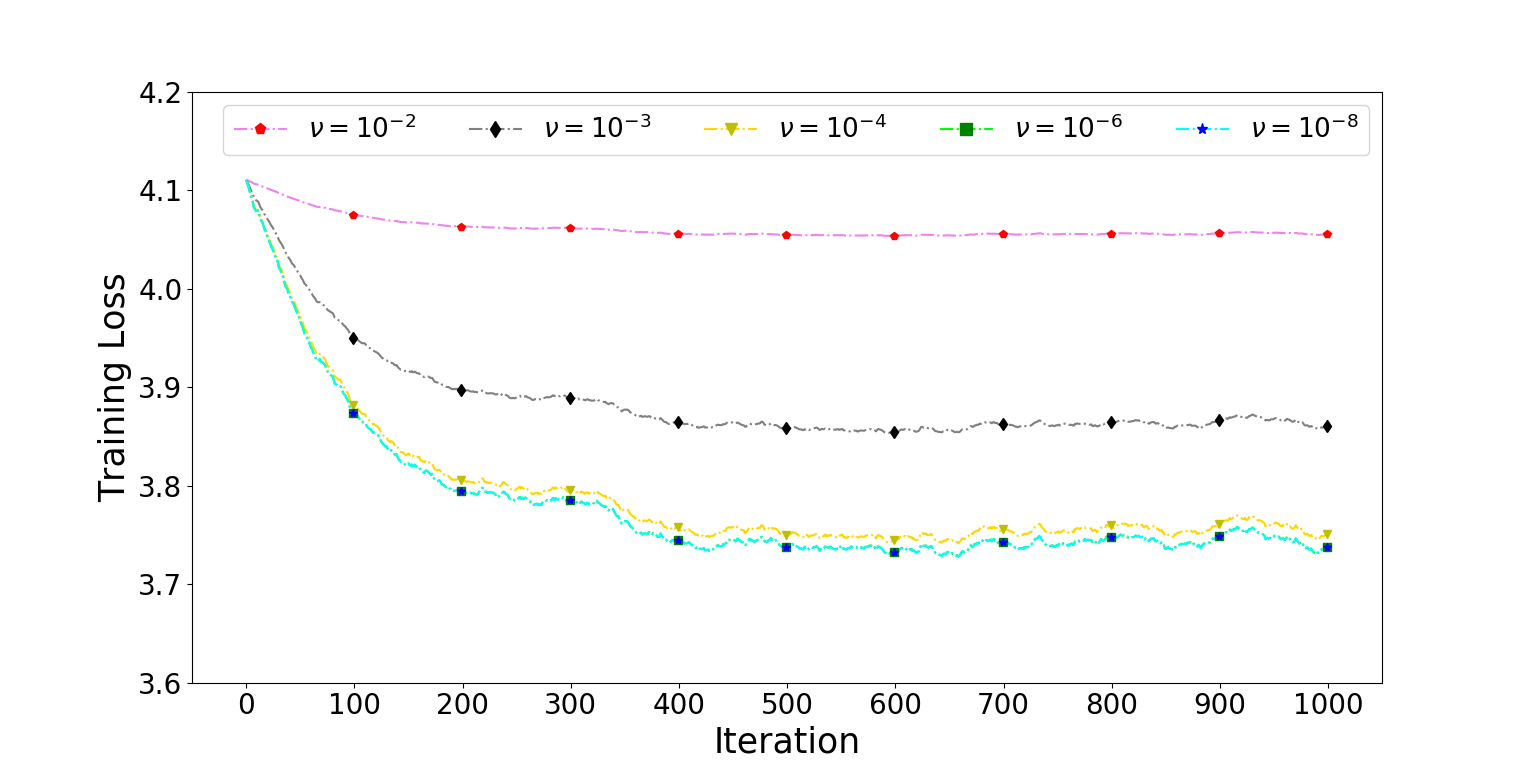
\includegraphics[width=0.46\textwidth, height=14em]{./figs/nu.png}\\
\vspace{2mm}
\parbox[c]{8.3cm}{\footnotesize{Fig.7.~}  The training loss V.S. iterations of ADMMiRNN on a text classification task with different $\nu$.}%\vspace*{.2mm}
\label{fig:nu}
\end{center}

No matter how the initialization changes, ADMMiRNN always gives a stable training process and promising results.
The results demonstrate that ADMMiRNN is a more stable training algorithm for RNN models than stochastic gradient algorithms.
\tabcolsep 6pt
%\cmidrule(l){2-4}%
\renewcommand\arraystretch{1.3}
\begin{center}
{\footnotesize{\bf Table 3.} \textcolor{red}{N}eeded \textcolor{red}{I}terations \textcolor{red}{W}hen the \textcolor{red}{A}ccuracy \textcolor{red}{R}eaches 1.0.}\\
\vspace{2mm}
\footnotesize{
\begin{tabular*}{\linewidth}{cccccc}\hline\hline\hline
$\rho_1$ & $\rho_2$ & $\rho_3$ & $r$ & training iterations & test iterations  \\
\hline
% \midrule
1 & 1 & 1 & 1   &  2   & 2    \\
0.1 & 1 & 1 & 1 &  2   & 2    \\
1 & 0.1 & 1 & 1 &  2   & 2   \\
1 &1 & 0.1 & 1  &  2   & 2    \\
1 &1 & 10  & 1   &  3   & 3   \\
1 & 1 & 10 & 10   &  11   & 11    \\
1 & 1 & 1 & 10  &  2   & 2    \\    
\hline\hline\hline
\end{tabular*}%\vspace*{.2mm}
%\\\vspace{1mm}\parbox{8.3cm}{Note: You may explain the meaning of some special format, e.g., in bold, and/or give the full names of the abbreviations used in the table whose full names have not presented in the text.}
}
\label{tab:hyper acc}
\end{center}
\subsection{Choices of Hyperparameters $\rho$s and $\nu$}
\subsubsection{varying $\rho$s}
In vanilla ADMM, the value of the penalty term is critical, and it may have negative effects on convergence.
In this subsection, we mainly try different hyperparameters in ADMMiRNN and evaluate how they influence the training process of ADMMiRNN. 
These results are summarized in Table~2 and Table~3.
Table~2 implies that $\rho_3$ determines the best result in ADMMiRNN.
More precisely, larger $\rho_3$ delays the convergence speed in ADMMiRNN.
However, if $\rho_3$ is too large, it may produce non-convergent results.
In Table~3, we present the needed iteration count when the accuracy is 1.0 in the training and test process.
When $\rho_3$ is 100, we need 11 iterations for the accuracy reaches 1.0 but we only need 2 iterations when $\rho_3=1$ or $\rho_3=10$.
Furthermore, it turns out that $\rho_1$ and $\rho_2$ account less in ADMMiRNN while $\rho_3$ plays a much more crucial role with regard to the property of convergence and its convergence speed.

\subsubsection{varying $\nu$}
In this subsection, we investigate the influence of $\nu$ in Eq.~\eqref{equ:phi}. In our experiments on a text data, we fix all the hyperparameters other than $\nu$ and set it $10^{-2}$, $10^{-3}$, $10^{-4}$, $10^{-6}$, $10^{-8}$ respectively. We display the curves corresponding to different values of $\nu$ in Fig.7.
Fig.7 suggests that larger $\nu$ produces a relatively worse convergence result in ADMMiRNN. Small $\nu$ can not only lead to a small loss but is also able to push the training process to converge fast. However, when $\nu$ is small enough, the influence on the convergence rate and convergent result is not obvious.  
\begin{center}
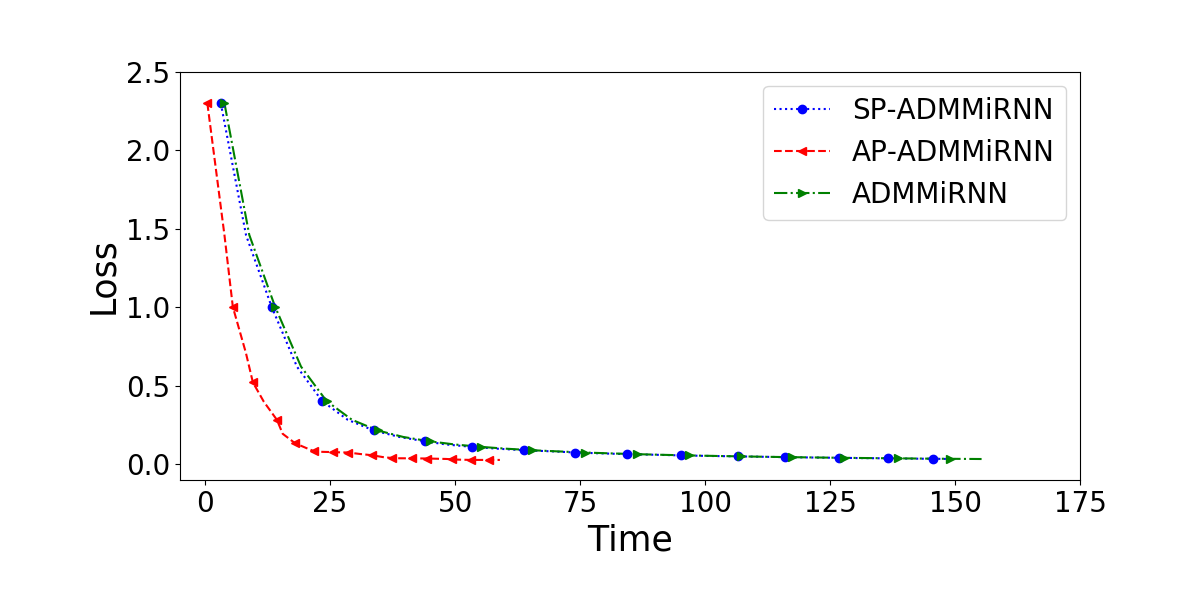
\includegraphics[width=0.46\textwidth, height=14em]{./figs/com_3worker.eps}\\
\vspace{2mm}
\parbox[c]{8.3cm}{\footnotesize{Fig.8.~}  The comparison of vanilla ADMMiRNN, SP-ADMMiRNN and AP-ADMMiRNN.}%\vspace*{.2mm}
\label{fig:comparasion of 3 workers}
\vspace{-1em}
\end{center}
\begin{center}
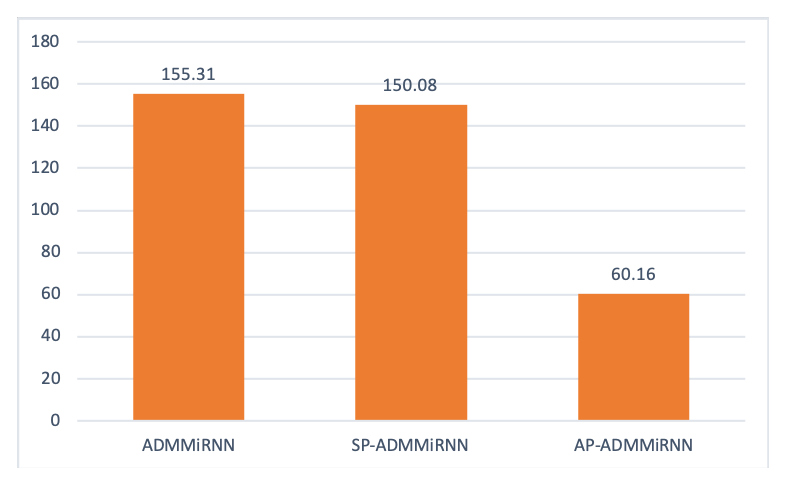
\includegraphics[width=0.4\textwidth, height=12em]{./figs/zhu.eps}\\
\vspace{2mm}
\parbox[c]{8.3cm}{\footnotesize{Fig.9.~}  Comparison of training time of different algorithms within 30 iterations.}%\vspace*{.2mm}
\label{fig:cost time 3 workers}
\end{center}
\begin{center}
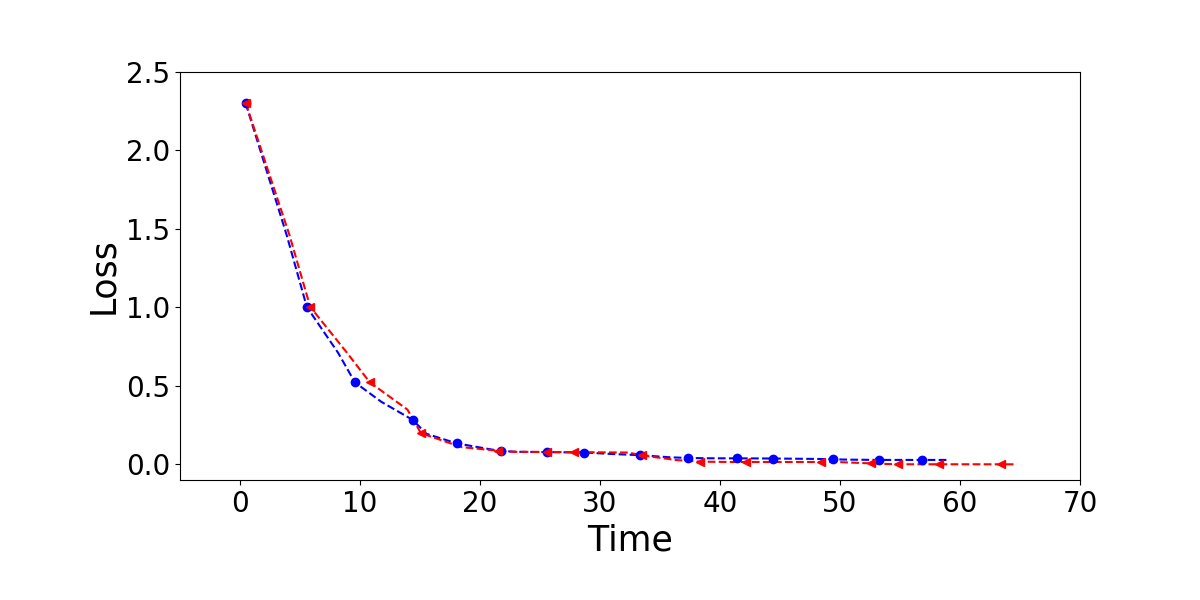
\includegraphics[width=0.46\textwidth, height=14em]{./figs/com_ave.eps}\\
\vspace{2mm}
\parbox[c]{8.3cm}{\footnotesize{Fig.10.~}  The results of utilizing \textit{average principle} or not.(the red curve iswith \textit{average principle} while the blue one is not).}%\vspace*{.2mm}
\label{fig:average principle}
\end{center}
\subsection{Paralleled Experiments}
To compare vanilla ADMMiRNN, SP-ADMMiRNN and AP-ADMMiRNN, we conduct several experiments on MNIST and present the experimental results in Fig.8. In this test, there are 3 workers in both SP-ADMMiRNN and AP-ADMMiRNN. Instead of using \textit{average principle}, we put the most time consuming parameters in one worker and the rest parameters are assigned to other workers.  We mainly focus on the training speed and the convergence rate of each scheme. It turns out that AP-ADMMiRNN converges much faster than vanilla ADMMiRNN and SP-ADMMiRNN.
To provide an intuitive comparison, we show the total training time of different algorithms on MNIST within 30 iterations in Fig.9. It is clear that AP-ADMMiRNN costs only about 60 seconds, less than ADMMiRNN and SP-ADMMiRNN.
When there are 3 workers, the cost time of vanilla ADMMiRNN is more than 2 times that of AP-ADMMiRNN. 
In Fig.8 and Fig.9, we also spot that SP-ADMMiRNN has a nearly the same curve as vanilla ADMMiRNN. This is because the parameters which are most time-consuming are assigned to the same worker. 

In order to verify the effectiveness of \textit{average principle}, we reassign the parameters to 3 workers and try to make the calculation time in each worker as similar as possible. This comparison is displayed in Fig.10. The red line is our experimental results with \textit{average principle} while the blue one is not. Fig.10 shows that using \textit{average principle} reduces the convergence speed a little but gets a lower loss. 
\begin{center}
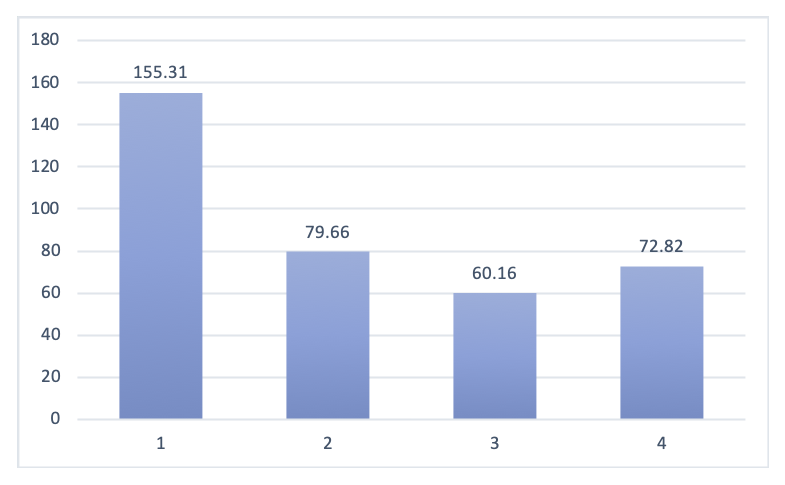
\includegraphics[width=0.46\textwidth, height=14em]{./figs/time.eps}\\
\vspace{2mm}
\parbox[c]{8.3cm}{\footnotesize{Fig.11.~}  The training time of different numbers of workers in AP-ADMMiNN within 30 iterations.}%\vspace*{.2mm}
\label{fig:multi time}
\end{center}
\begin{center}
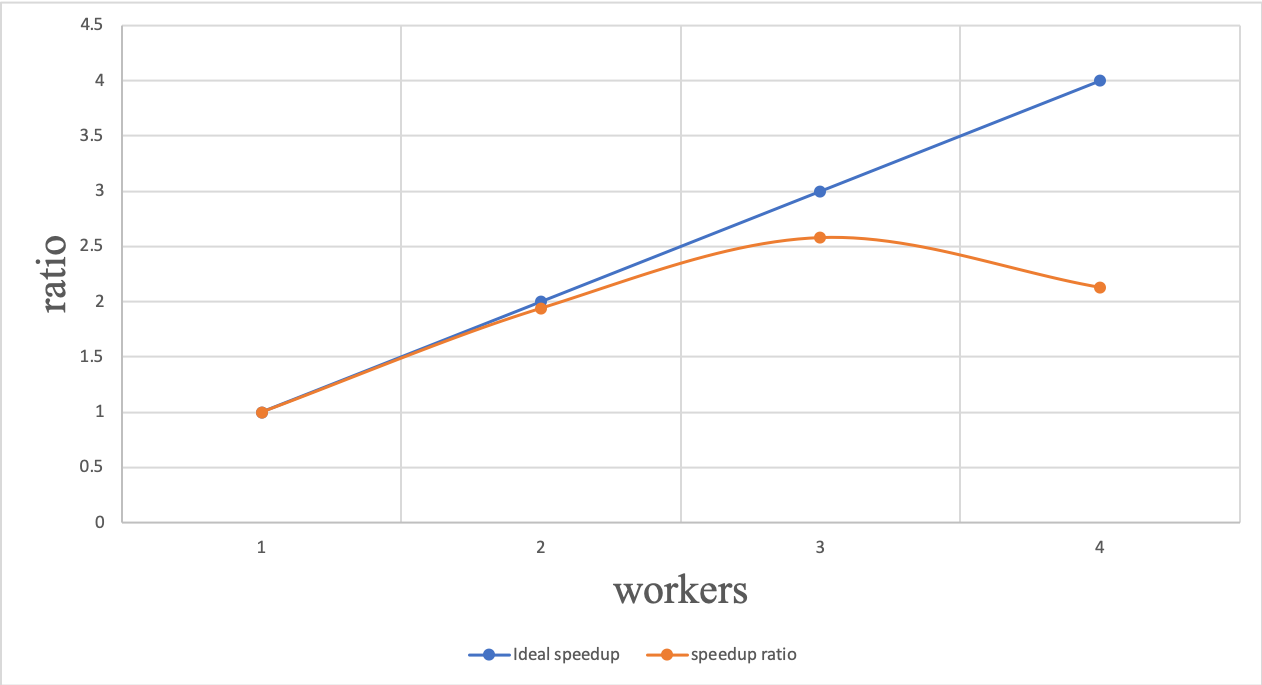
\includegraphics[width=0.46\textwidth, height=14em]{./figs/ratio.eps}\\
\vspace{2mm}
\parbox[c]{8.3cm}{\footnotesize{Fig.12.~}  The ideal and actual speedup ratio of different numbers of workers in AP-ADMMiRNN.}%\vspace*{.2mm}
\label{fig:ratio}
\end{center}
In addition, we further investigate how the number of workers incluence training performance in AP-ADMMiRNN. Those experiments are performed on 1, 2, 3, 4 workers respectively and results are shown in Fig.11 and Fig.12. In both Fig.11 and Fig.12, the X axis stands for the number of workers in AP-ADMMiRNN. In Fig.11, the Y axis represents the cost time while the Y axis in Fig.12 denotes the speedup ratio. In Fig.12, the blue line is the ideal speedup ratio and the orange one is the actual speedup ratio.
We observe that there is a clear speedup when the number workers increase from 1 to 3. And the difference between actual and ideal speedup ratio is going up. 
When there are 4 workers in our test, the training time costs more than that of 3 workers and the speedup is worse. This is because when there are too many workers and the parameters are assigned so that the master keeps receiving updates, which causes blocks in the master and brings extra time overhead.  

\section{Conclusion}\label{sec:conclusion}
In this paper, we proposed a new framework to train RNN tasks, namely ADMMiRNN. 
Since it is challenging to train RNNs with ADMM directly, we set up ADMMiRNN on the foundation of the expanded form of RNNs. 
The convergence analysis of ADMMiRNN is presented, and ADMMiRNN could achieve a convergence rate of $O(1/T)$. 
We further conduct several experiments on real-world datasets based on our theoretical analysis. 
% We compare ADMMiRNN with several popular optimizers. 
Experimental results of comparisons regarding ADMMiRNN and several popular optimizers manifest that ADMMiRNN converges faster than these gradient-based optimizers.
Besides, it presents a much more stable process than them.
% It is obvious that ADMMiRNN not only gives a promising convergent result, but also . 
To the best of our knowledge, we are the first to apply ADMM into RNN tasks, and present theoretical analysis and ADMMiRNN is the first to alleviate the \textit{vanishing} and \textit{exploding} gradients problem and the sensitivity of RNN models to initializations at the same time.
In conclusion, ADMMiRNN is a promising tool to train RNN models. % What's more, ADMMiRNN is easy to be achieved in a distributed way. 
Another important contribution of our work is AP-ADMMiRNN. We train ADMMiRNN in an asynchronous parallel way and make a fair comparison among vanilla ADMMiRNN, SP-ADMMiRNN and AP-ADMMiRNN. Experiments demonstrate that AP-ADMMiRNN converges faster than vanilla ADMMiRNN and SP-ADMMiRNN.
Further experiments illustrate that the number of workers is also critical concerning the speedup ratio, which means we cannot make the master too busy for the sake of better training performance.

%\section*{Acknowledgment}
%
%This work is partially sponsored by the National Natural Science Foundation of China under Grant No. 61806216, 61702533, 61932001, 61872376 and 61701506.

\appendix
\section{appendix A}\label{appendix A}
% \section{Appendix A}\label{appendix A}
\subsection{Update $w$}
%As for the update of $w$ in Eq.~\eqref{equ:lagrangian}, it follows
%% at iteration $k$, it is updated as follows:
%% \begin{equation}\nonumber
%%     w^{\Tilde{k}} \leftarrow \arg\min \mathcal{L}_{\rho_1,\rho_2,\rho_3}(u^{\Tilde{k}},w,b^k,a^k,s^k,v^k,c^k,o^k).
%% \end{equation}
%% which is equivalent to the following form:
%\begin{equation}\label{equ:update_wt}
%    w^{\Tilde{k}} \leftarrow \arg\min \Omega(w) + \phi(u^{\Tilde{k}},w,b^k,a^k,s^k,v^k,c^k,o^k).
%\end{equation}

Similar as the update of $u$ in Section~\ref{sec:update_u}, 
we also define $\textbf{G}=rI_{d}-\rho_1 s_{t-1}^Ts_{t-1}$ and use with linearized proximal point method, then the update of $w$ is transformed into
\begin{equation}
    \begin{aligned}\label{equ:update_w}
        w^{\Tilde{k}} \leftarrow & \arg\min \Omega(w) \frac{Nr}{2}\|w-w^k\|^2+\nu(w-w^k)^T\sum_{t=1}^{N-1}[(s_{t-1}^k)^T\\
        & (a_t^k-u^kx_t^k-w^ks_{t-1}^k-b^k)]+\rho_1(w-w^k)^T[(s_{N-1}^k)^T  \\
        & (a_N^k-u^kx_N^k-w^ks_{N-1}^k-b^k-\lambda_1^k/\rho_1)].  \\
    \end{aligned}
\end{equation}

\subsection{Update $b$}
As far as $b$ is concerned, it is updated by 
% has a similar updating rule.
% \begin{equation}\nonumber
%     b^{\Tilde{k}} \leftarrow \arg\min \mathcal{L}_{\rho_1,\rho_2,\rho_3}(u^{\Tilde{k}},w^{\Tilde{k}},b,a^k,s^k,v^k,c^k,o^k),
% \end{equation}
% and the updating rule of $b$ is transformed into:
\begin{equation}\label{equ:update_bt}
    b^{\Tilde{k}} \leftarrow \arg\min \phi(u^{\Tilde{k}},w^{\Tilde{k}},b,a^k,s^k,v^k,c^k,o^k).
\end{equation}

\subsection{Update $v$}
% We spot that $v$ and $s_t$ are not decoupled in Eq.~\eqref{equ:phi}.
% Therefore, 
% to avoid high computational complexity, we adopt a similar way as that in updating $u$ and $w$. 
% The parameter $v$ is updated as follows:
% \begin{equation}\nonumber
%     v^{\Tilde{k}} \leftarrow \arg\min \mathcal{L}_{\rho_1,\rho_2,\rho_3}(u^{\Tilde{k}},w^{\Tilde{k}},b^{\Tilde{k}},a^{\Tilde{k}},s^{\Tilde{k}},v,c^k,o^k),
% \end{equation}
% Equally, adapt the following form and update $v_t$.
% \begin{equation}\nonumber
%     v^{\Tilde{k}} \leftarrow \arg\min \phi(u^{\Tilde{k}},w^{\Tilde{k}},b^{\Tilde{k}},a^{\Tilde{k}},s^{\Tilde{k}},v,c^k,o^k).
% \end{equation}
Similar as aforementioned, the update rule for $v$ is 
\begin{equation}\label{equ:update_vt}
    \begin{aligned}
        v^{\Tilde{k}} \leftarrow & \arg\min \frac{Nr}{2}\|v-v^k\|^2+\nu(v-v^k)^T\sum_{t=1}^{N-1}[(s_t^k)^T(o_t^k\\
        &  - v^ks_t^k-c^k)]+\rho_3(v-v^k)^T[(s_N^k)^T(o_N^k-v^ks_N^k-    \\
        & c^k -\lambda_1^k/\rho_3)].  \\
    \end{aligned}
\end{equation}


\subsection{Update $c$}
The parameter $c$ is quite simple, which is updated as follows:
% \begin{equation}\nonumber
%     c^{\Tilde{k}} \leftarrow \arg\min \mathcal{L}_{\rho_1,\rho_2,\rho_3}(u^{\Tilde{k}},w^{\Tilde{k}},b^{\Tilde{k}},a^{\Tilde{k}},s^{\Tilde{k}},v^{\Tilde{k}},c,o^k),
% \end{equation}
% which is equivalent to the following form:
\begin{equation}\label{equ:update_ct}
    c^{\Tilde{k}} \leftarrow \arg\min \phi(u^{\Tilde{k}},w^{\Tilde{k}},b^{\Tilde{k}},a^{\Tilde{k}},s^{\Tilde{k}},v^{\Tilde{k}},c,o^k).
\end{equation}
\subsection{Update $o$}
Finally, we update $o_t$.
%through:
%% \begin{equation}\nonumber
%%     o_t^{\Tilde{k}} \leftarrow \arg\min \mathcal{L}_{\rho_1,\rho_2,\rho_3}(u^{\Tilde{k}},w^{\Tilde{k}},b^{\Tilde{k}},a^{\Tilde{k}},s^{\Tilde{k}},v^{\Tilde{k}},c^{\Tilde{k}},o_t),
%% \end{equation}
%% which is equivalent to the following form:
%\begin{equation}\nonumber
%    o_t^{\Tilde{k}} \leftarrow \arg\min R(o) + \phi(u^{\Tilde{k}},w^{\Tilde{k}},b^{\Tilde{k}},a^{\Tilde{k}},s^{\Tilde{k}},v^{\Tilde{k}},c^{\Tilde{k}},o_t).
%\end{equation}
It has to be noted that each $o_t$ is also updated separably. If $t<N$, 
\begin{equation}\label{equ:update_ot}
    \begin{aligned}
        o_t^{\Tilde{k}} \leftarrow \arg\min R(o)+\frac{\nu}{2}\|o_t^k-v^ks_t^k-c^k\|^2 .
    \end{aligned}
\end{equation}
If $t=N$,
\begin{equation}\label{equ:update_oN}
    \begin{aligned}
        o_N^{\Tilde{k}} \leftarrow \arg\min R(o)+\frac{\rho_3}{2}\|o_N^k-v^ks_N^k-c^k-\lambda_3^k/\rho_3\|^2 .
    \end{aligned}
\end{equation}

%\setcounter{figure}{1}
%\begin{figure*}[!htb]
%\centering
%  \subfigure[]{
%    \includegraphics[width=6cm,height=2cm]{photo.eps}}
%  \subfigure[]{
%    \includegraphics[width=6cm,height=2cm]{photo.eps}}
%  \caption{Example for inserting a two-column wide figure. (a) Title of sub-figure (a). (b) Title of sub-figure (b).}
%\end{figure*}
%\baselineskip=18pt plus.2pt minus.2pt
%\parskip=0pt plus.2pt minus0.2pt

%\tabcolsep 12pt
%%\cmidrule(l){2-4}%
%\renewcommand\arraystretch{1.3}
%\begin{center}
%{\footnotesize{\bf Table 1.} \textcolor{red}{C}aption of \textcolor{red}{T}his \textcolor{red}{O}ne-\textcolor{red}{C}olumn \textcolor{red}{W}ide \textcolor{red}{T}able}\\
%\vspace{2mm}
%\footnotesize{
%\begin{tabular*}{\linewidth}{c}\hline\hline\hline
%\\\hline
%\\
%\\
%\\\hline\hline\hline
%\end{tabular*}%\vspace*{.2mm}
%\\\vspace{1mm}\parbox{8.3cm}{Note: You may explain the meaning of some special format, e.g., in bold, and/or give the full names of the abbreviations used in the table whose full names have not presented in the text.}
%}
%\end{center}
%
%\setcounter{table}{1}
%\tabcolsep 9pt
%%\cmidrule(l){2-4}
%\renewcommand\arraystretch{1.3}
%\begin{table*}[!htb]
%\centering
%\caption{\label{3} \textcolor{red}{C}aption of \textcolor{red}{T}his \textcolor{red}{T}able}\vspace{-2mm}
%{\footnotesize
%\begin{tabular*}{\linewidth}{c}\hline\hline\hline
%\\\hline
%\\
%\\
%\\\hline\hline\hline
%\end{tabular*}%\vspace*{.2mm}
%%\\\vspace{1mm}\parbox{17.5cm}{}
%}
%\end{table*}
%\baselineskip=18pt plus.2pt minus.2pt
%\parskip=0pt plus.2pt minus0.2pt


\begin{thebibliography}{99}
\footnotesize
\itemsep=-3pt plus.2pt minus.2pt
\baselineskip=13pt plus.2pt minus.2pt

\bibitem{bengio1994learning}
Bengio, Y., Simard, P., Frasconi, P., et al.: Learning long-term dependencies with gradient descent is difficult. IEEE transactions on neural networks \textbf{5}(2), 157--166 (1994)

\bibitem{boyd2011distributed}
Boyd, S., Parikh, N., Chu, E., Peleato, B., Eckstein, J., et al.: Distributed optimization and statistical learning via the alternating direction method of multipliers. Foundations and Trends{\textregistered} in Machine learning \textbf{3}(1), 1--122 (2011)

\bibitem{duchi2011adaptive}
Duchi, J., Hazan, E., Singer, Y.: Adaptive subgradient methods for online learning and stochastic optimization. Journal of Machine Learning Research \textbf{12}(Jul), 2121--2159 (2011)

\bibitem{elman1990finding}
Elman, J.L.: Finding structure in time. Cognitive science \textbf{14}(2), 179--211 (1990)

\bibitem{gabay1983augmented}
Gabay, D.: Augmented lagrangian methods: applications to the solution of boundary-value problems, chapter applications of the method of multipliers to
variational inequalities. North-Holland, Amsterdam \textbf{3}, 4 (1983)

\bibitem{mikolov2010recurrent}
Kombrink, S., Mikolov, T., Karafi${\acute a}$t, M., \& Burget, L. (2011). 
Recurrent neural network based language modeling in meeting recognition. In {\it Twelfth annual conference of the international speech communication association}.

\bibitem{gabay1976dual}
Gabay, D., Mercier, B.: A dual algorithm for the solution of nonlinear variational problems via finite element approximation. Computers \& mathematics with applications \textbf{2}(1), 17--40 (1976)

% \bibitem{GhadimiMini}
% Ghadimi, S., Lan, G., Zhang, H.: Mini-batch stochastic approximation methods for nonconvex stochastic composite optimization. Mathematical Programming \textbf{155}(1--2), 267--305

\bibitem{glowinski1989augmented}
Glowinski, R., Le Tallec, P.: Augmented Lagrangian and operator-splitting methods in nonlinear mechanics, vol. 9. SIAM (1989)

\bibitem{goldfarb2014robust}
Goldfarb, D., Qin, Z.: Robust low-rank tensor recovery: Models and algorithms. SIAM Journal on Matrix Analysis and Applications \textbf{35}(1), 225--253 (2014)

\bibitem{goodfellow2016deep}
Goodfellow, I., Bengio, Y., Courville, A.: Deep learning. MIT press (2016)

\bibitem{graves2007multi}
Graves, A., Fern{\'a}ndezz, S., Schmidhuber, J.: Multi-dimensional recurrent neural networks. In: International conference on artificial neural networks. pp. 549--558. Springer (2007)

\bibitem{hochreiter1997long}
Hochreiter, S., Schmidhuber, J.: Long short-term memory. Neural computation \textbf{9}(8), 1735--1780 (1997)

\bibitem{Kingma2014Adam}
Kingma, D., Ba, J.: Adam: A method for stochastic optimization. Computer Science (2014)

\bibitem{krizhevsky2012imagenet}
Krizhevsky, A., Sutskever, I., Hinton, G.E.: Imagenet classification with deep convolutional neural networks. In: Advances in neural information processing systems. pp. 1097--1105 (2012)

\bibitem{Lai2015TC}
Lai, S., Xu, L., Liu, K., Zhao, J.: Recurrent convolutional neural networks for text classification. In: AAAI. vol. 333, pp. 2267--2273 (2015)

\bibitem{lecun2015deep}
LeCun, Y., Bengio, Y., Hinton, G.: Deep learning. nature \textbf{521}(7553), 436--444 (2015)

\bibitem{lecun1998gradient}
LeCun, Y., Bottou, L., Bengio, Y., Haffner, P., et al.: Gradient-based learning applied to document recognition. Proceedings of the IEEE \textbf{86}(11), 2278--2324 (1998)

\bibitem{monteiro2010iteration}
Monteiro, R.D., Svaiter, B.F.: Iteration-complexity of block-decomposition algorithms and the alternating minimization augmented lagrangian method. Manuscript, School of Industrial and Systems Engineering, Georgia Institute of Technology, Atlanta, GA pp. 30332--0205 (2010)

\bibitem{nair2010rectified}
Nair, V., Hinton, G.E.: Rectified linear units improve restricted boltzmann machines. In: Proceedings of the 27th international conference on machine learning
(ICML-10). pp. 807--814 (2010)

\bibitem{Nguyen2016JRNN}
Nguyen, T.H., Cho, K., Grishman, R.: Joint event extraction via recurrent neural
networks. In: Proceedings of the 2016 Conference of the North American Chapter of the Association for Computational Linguistics: Human Language Technologies. pp. 300--309 (2016)

\bibitem{pascanu2013difficulty}
Pascanu, R., Mikolov, T., Bengio, Y.: On the difficulty of training recurrent neural networks. In: International conference on machine learning. pp. 1310--1318 (2013)

\bibitem{qian1999momentum}
Qian, N.: On the momentum term in gradient descent learning algorithms. Neural
networks \textbf{12}(1), 145--151 (1999)

\bibitem{robbins1951stochastic}
Robbins, H., Monro, S.: A stochastic approximation method. The annals of math-
ematical statistics pp. 400--407 (1951)

\bibitem{rockafellar1976monotone}
Rockafellar, R.T.: Monotone operators and the proximal point algorithm. SIAM
journal on control and optimization \textbf{14}(5), 877--898 (1976)

\bibitem{masuyama2018modal}
Masuyama, Y., Kusano, T., Yatabe, K., \& Oikawa, Y. (2018, April). Modal decomposition of musical instrument sound via alternating direction method of multipliers. In {\it 2018 IEEE International Conference on Acoustics, Speech and Signal Processing (ICASSP)} (pp. 631-635). IEEE.

\bibitem{sun2018iteratively}
Sun, T., Jiang, H., Cheng, L., Zhu, W.: Iteratively linearized reweighted alter-
nating direction method of multipliers for a class of nonconvex problems. IEEE Transactions on Signal Processing \textbf{66}(20), 5380--5391 (2018)

\bibitem{sutskever2013importance}
Sutskever, I., Martens, J., Dahl, G., Hinton, G.: On the importance of initialization and momentum in deep learning. In: International conference on machine learning. pp. 1139--1147 (2013)

\bibitem{taylor2016training}
Taylor, G., Burmeister, R., Xu, Z., Singh, B., Patel, A., Goldstein, T.: Training neural networks without gradients: A scalable admm approach. In: International conference on machine learning. pp. 2722--2731 (2016)

\bibitem{tieleman2012lecture}
Tieleman, T., Hinton, G.: Lecture 6.5-rmsprop, coursera: Neural networks for machine learning. University of Toronto, Technical Report (2012)

\bibitem{wang2019admm}
Wang, J., Yu, F., Chen, X., Zhao, L.: Admm for efficient deep learning with global convergence. In: Proceedings of the 25th ACM SIGKDD International Conference on Knowledge Discovery \& Data Mining. pp. 111--119 (2019)

\bibitem{wang2019multi}
Wang, J., Zhao, L., Wu, L.: Multi-convex inequality-constrained alternating direction method of multipliers. arXiv preprint arXiv:1902.10882 (2019)

\bibitem{ouyang2013stochastic}
Ouyang, H., He, N., Tran, L., \& Gray, A. (2013, February). Stochastic alternating direction method of multipliers. In {\it International Conference on Machine Learning} (pp. 80-88).

\bibitem{zhong2014fast}
Zhong, W., Kwok, J.: Fast stochastic alternating direction method of multipliers. In: International Conference on Machine Learning. pp. 46--54 (2014)

\bibitem{Saeed1} 
Saeed G., Guanghui L.: Stochastic first- and zeroth-order methods for nonconvex stochastic programming. \textit{SIAM Journal on Optimization}, 23(4):2341-2368, 2013a. doi: 10.1137/ 120880811.

\bibitem{Saeed2}
Saeed G., Guanghui L., Hongchao Z. :Mini-batch stochastic approximation methods
for nonconvex stochastic composite optimization. \textit{Mathematical Programming}, 155(1-2):267-305,
2014.

\bibitem{zou2019sufficient}
Zou, F., Shen, L., Jie, Z., Zhang, W., Liu, W.: A sufficient condition for convergences of adam and rmsprop. In: Proceedings of the IEEE Conference on Computer Vision and Pattern Recognition. pp. 11127--11135 (2019)

\bibitem{chang2016asynchronous}
Chang, T. H., Hong, M., Liao, W. C., \& Wang, X. (2016). Asynchronous distributed ADMM for large-scale optimization-Part I: Algorithm and convergence analysis. IEEE Transactions on Signal Processing, 64(12), 3118--3130.

\bibitem{wei2013}
Wei, E., \& Ozdaglar, A. (2013, December). On the o (1= k) convergence of asynchronous distributed alternating direction method of multipliers. In {\it 2013 IEEE Global Conference on Signal and Information Processing} (pp. 551-554). IEEE.

\bibitem{dodds2006popular}
Dodds, K. (2006). Popular geopolitics and audience dispositions: James Bond and the internet movie database (IMDb). {\it Transactions of the Institute of British Geographers}, 31(2), 116-130.

% \bibitem{1}Sayah J Y, Kime C R. Test scheduling in high performance VLSI system implementations. {\it IEEE Trans. Computers}, 1992, 41(1): 52-67. [\textcolor{blue}{example for journal paper}]

% \bibitem{2} Gordon Plotkin. A semantics for type checking. In {\it Lecture Notes in Computer Science 526,} Ito T, Meyer A R (eds.), Springer-Verlag, 1991, pp.1-17. [\textcolor{blue}{example for book chapter}]


% \bibitem{3} Geddes K O, Czapor S R, Labahn G. Algorithms for Computer Algebra. Boston: Kluwer, 1992. [\textcolor{blue}{example for book}]

% \bibitem{4} Kwan A W, Bic L. Distributed memory computers. In {\it Proc. the 6th Int. Parallel Processing Symp.}, March 1992, pp.10-17. [\textcolor{blue}{example for conference}]

% \bibitem{5} Harris M J. Real-time cloud simulation and rendering [Ph.D. Thesis]. Department of Computer Science, The University of North Carolina at Chapel Hill, 2003. [\textcolor{blue}{example for thesis}]

% \bibitem{6} Jurczyk M, Coldwind G. Identifying and ex-ploiting windows kernel race conditions via mem-ory access patterns. Technical Report, Google Re-search, 2013. http://pdfs.semanticscholar.org/ca60/2e7193f159a56a3559-f08b677abfba60beb2.pdf, Mar. 2018. [\textcolor{blue}{example for technical report}]

% \bibitem{7} Gipp B, Meuschke N, Gernandt A. Decentra-lized trusted timestamping using the crypto cur-rency Bitcoin. arXiv:1502.04015, 2015. https://arxiv.org/abs/1502.04015, May. 2018. [\textcolor{blue}{example for ar-Xiv document}]

% \bibitem{8} Tong Y, Chen L, Zhou Z, JagadishH V, Shou L, Lv W. SLADE: A smart large-scale task decomposer in crowdsourcing. {\it IEEE Transactions on Knowledge and Data Engineering}. doi:10.1109/TKDE.2018.2797962. (preprint) [\textcolor{blue}{example for preprint}]

\end{thebibliography}

\label{last-page}
\end{multicols}
\label{last-page}
\end{document}

